% **************************************************************************************************************
% A Classic Thesis Style
% An Homage to The Elements of Typographic Style
%
% Copyright (C) 2012 Andr\'e Miede http://www.miede.de
%
% If you like the style then I would appreciate a postcard. My address 
% can be found in the file ClassicThesis.pdf. A collection of the 
% postcards I received so far is available online at 
% http://postcards.miede.de
%
% License:
% This program is free software; you can redistribute it and/or modify
% it under the terms of the GNU General Public License as published by
% the Free Software Foundation; either version 2 of the License, or
% (at your option) any later version.
%
% This program is distributed in the hope that it will be useful,
% but WITHOUT ANY WARRANTY; without even the implied warranty of
% MERCHANTABILITY or FITNESS FOR A PARTICULAR PURPOSE.  See the
% GNU General Public License for more details.
%
% You should have received a copy of the GNU General Public License
% along with this program; see the file COPYING.  If not, write to
% the Free Software Foundation, Inc., 59 Temple Place - Suite 330,
% Boston, MA 02111-1307, USA.
%
% **************************************************************************************************************
% Note:
%    * You must not use "u etc. in strings/commands that will be spaced out (use \"u or real umlauts instead)
%    * New enumeration (small caps): \begin{aenumerate} \end{aenumerate}
%    * For margin notes: \marginpar or \graffito{}
%    * Do not use bold fonts in this style, it is designed around them
%    * Use tables as in the examples
%    * See classicthesis-preamble.sty for useful commands
% **************************************************************************************************************
% To Do:
%		 * [high] Check this out: http://www.golatex.de/koma-script-warnung-in-verbindung-mit-listings-package-t2058.html
%    * [medium] mathbb in section-titles/chapter-titles => disappears somehow in headlines!!!
% **************************************************************************************************************
\documentclass[ twoside,openright,titlepage,numbers=noenddot,headinclude,%1headlines,% letterpaper a4paper
                footinclude=true,cleardoublepage=plain,abstractoff, % <--- obsolete, remove (todo)
                BCOR=5mm,paper=a4,fontsize=11pt,%11pt,a4paper,%
                english,
                dottedtoc, % adicionar pontinhos na lista de conteúdos
                ]{scrreprt}


% UTF-8 support with latin9 (ISO-8859-9) = latin1+"Euro sign"
\PassOptionsToPackage{utf8}{inputenc}   
\usepackage{inputenc}  
 
% ****************************************************************************************************
% Personal data and user ad-hoc commands
% ****************************************************************************************************
\newcommand{\myTitle}{AUTOPSY – Enhanced distributed forensic analysis\xspace}
\newcommand{\myDegree}{Mestrado em Cibersegurança e Informática Forense\xspace}
\newcommand{\myNameOne}{Pedro Henrique Gaspar Cordeiro Ferreira\xspace}
\newcommand{\myNumber}{2180078}


\newcommand{\company}{VOID SOFTWARE, S.A.}
\newcommand{\myProf}{Marisa da Silva Maximiano}

\newcommand{\myProfOne}{Professora Doutora Marisa da Silva Maximiano  \href{mailto:marisa.maximiano@ipleiria.pt}{(marisa.maximiano@ipleiria.pt)}\xspace}
% \newcommand{\myProfTwo}{Professor Doutor XXXX XXXXX XXXXX \href{mailto:xxxxxx@ipleiria.pt}{(xxxxxx@ipleiria.pt)}\xspace}

\newcommand{\myFaculty}{Politécnico de Leiria\xspace}
\newcommand{\mySchool}{Escola Superior de Tecnologia e Gestão\xspace}
\newcommand{\myDepartment}{Departamento de Engenharia Informática\xspace}
\newcommand{\myLocation}{Leiria\xspace}

\newcommand{\myTime}{31 de Julho de 2020\xspace}
\newcommand{\mySchoolYear}{2019 -- 2020\xspace}
\newcommand{\myVersion}{version 1.0\xspace}            
                
                
%*******************************************************
% Note: Make all your adjustments in here
%*******************************************************
% ****************************************************************************************************
% classicthesis-config.tex 
% formerly known as loadpackages.sty, classicthesis-ldpkg.sty, and classicthesis-preamble.sty 
% Use it at the beginning of your ClassicThesis.tex, or as a LaTeX Preamble 
% in your ClassicThesis.{tex,lyx} with \input{classicthesis-config}
% ****************************************************************************************************  
% If you like the classicthesis, then I would appreciate a postcard. 
% My address can be found in the file ClassicThesis.pdf. A collection 
% of the postcards I received so far is available online at 
% http://postcards.miede.de
% ****************************************************************************************************

% ****************************************************************************************************
% 1. Configure classicthesis for your needs here, e.g., remove "drafting" below 
% in order to deactivate the time-stamp on the pages
% ****************************************************************************************************
\PassOptionsToPackage{
                    eulerchapternumbers,
                    drafting, % comentar para remover a linha com a versão
                    pdfspacing,
                    %floatperchapter,
                    %linedheaders,%
                    subfig,beramono,
                    eulermath,
                    parts
                    }{classicthesis}
% Available options for classicthesis.sty 
% (see ClassicThesis.pdf for more information):
% drafting
% parts nochapters linedheaders
% eulerchapternumbers beramono eulermath pdfspacing minionprospacing
% tocaligned dottedtoc manychapters
% listings floatperchapter subfig
% ********************************************************************

% ********************************************************************
% Triggers for this config
% ******************************************************************** 
\usepackage{ifthen}
\newboolean{enable-backrefs} % enable backrefs in the bibliography
\setboolean{enable-backrefs}{false} % true false
% ****************************************************************************************************


% ********************************************************************
% Setup, finetuning, and useful commands
% ********************************************************************
\newcounter{dummy} % necessary for correct hyperlinks (to index, bib, etc.)
\newlength{\abcd} % for ab..z string length calculation
\providecommand{\mLyX}{L\kern-.1667em\lower.25em\hbox{Y}\kern-.125emX\@}
\newcommand{\ie}{\textit{i.\,e.}\xspace}
\newcommand{\Ie}{\textit{I.\,e.}\xspace}
\newcommand{\eg}{\textit{e.\,g.}\xspace}
\newcommand{\Eg}{\textit{E.\,g.}\xspace} 
\newcommand{\etc}{\textit{etc}\xspace} 


% ****************************************************************************************************
% \DeclareTextFontCommand{\code}{\fontfamily{pcr}\scriptsize}


% ****************************************************************************************************
% 3. Loading some handy packages
% ****************************************************************************************************
% ******************************************************************** 
% Packages with options that might require adjustments
% ******************************************************************** 

\PassOptionsToPackage{portuguese}{babel}
\usepackage{babel}

 
%%%%%%%%%%%%%%%%%%%%%%%%%%%%%%%%%%%%%%%%%%%%%%%%%%%%%
% Bibliografia
%%%%%%%%%%%%%%%%%%%%%%%%%%%%%%%%%%%%%%%%%%%%%%%%%%%%%
% package recomendada para usar com o biblatex
\usepackage{csquotes}

% carrega a package biblatex
\usepackage[
    backend=biber,    % usar o biber para processar
    style=authoryear, % estilo de citação
    sortcites=true,
    maxcitenames=2,   % a partir de 2 escreve "et al."
]{biblatex} 

% para adicionar uma vírgula antes do ano: (Dirac, 1981)
\renewcommand*{\nameyeardelim}{\addcomma\space}

%  dica: configurar o kile para reconhecer os comandos:
%    \parencite{bibkey}
%    \textcite{bibkey}
%    \citeauthor{bibkey}
%    \citetitle{bibkey}
%    
%    Settingis -> Configure Kile -> Latex/General -> Commands/Configure -> Commands/Citation -> add
%%%%%%%%%%%%%%%%%%%%%%%%%%%%%%%%%%%%%%%%%%%%%%%%%%%%%
 
\usepackage{float}

\PassOptionsToPackage{fleqn}{amsmath}		% math environments and more by the AMS 
\usepackage{amsmath}

\usepackage{multirow}
 
%******************************************************************** 
% General useful packages
%******************************************************************** 
\PassOptionsToPackage{T1}{fontenc} % T2A for cyrillics
\usepackage{fontenc}

\usepackage{textcomp} % fix warning with missing font shapes
\usepackage{scrhack} % fix warnings when using KOMA with listings package          
\usepackage{xspace} % to get the spacing after macros right  
\usepackage{mparhack} % get marginpar right
% \usepackage{fixltx2e} % fixes some LaTeX stuff 

\PassOptionsToPackage{printonlyused,smaller}{acronym}
\usepackage{acronym} % nice macros for handling all acronyms in the thesis

%\renewcommand*{\acsfont}[1]{\textssc{#1}} % for MinionPro
\newcommand{\bflabel}[1]{{#1}\hfill} % fix the list of acronyms
%****************************************************************************************************


%****************************************************************************************************
% 4. Setup floats: tables, (sub)figures, and captions
%****************************************************************************************************
\usepackage{tabularx} % better tables
    \setlength{\extrarowheight}{3pt} % increase table row height
\newcommand{\tableheadline}[1]{\multicolumn{1}{c}{\spacedlowsmallcaps{#1}}}
\newcommand{\tableheadlineR}[1]{\multicolumn{1}{r}{\spacedlowsmallcaps{#1}}}
\newcommand{\myfloatalign}{\centering} % to be used with each float for alignment
\usepackage{caption}
\captionsetup{format=hang,font=small}
\usepackage{subfig}  
% ****************************************************************************************************


%----------------------------------------------------------
% Filipius's famous "issue" command (Patricio, 2016-08-03)
%----------------------------------------------------------
\newcommand{\issue}[1] { {\footnotesize\textbf{
    \begin{center}
      \begin{tabular}{|c|}
        \hline
	\parbox[c]{\textwidth}{
          \medskip
          #1
          \medskip} \\
        \hline
      \end{tabular}
    \end{center}
  }
 }
}


% ****************************************************************************************************
% 6. PDFLaTeX, hyperreferences and citation backreferences
% ****************************************************************************************************
% ********************************************************************
% Using PDFLaTeX
% ********************************************************************
\PassOptionsToPackage{pdftex,hyperfootnotes=false,pdfpagelabels}{hyperref}
	\usepackage{hyperref}  % backref linktocpage pagebackref
\pdfcompresslevel=9
\pdfadjustspacing=1 
\PassOptionsToPackage{pdftex}{graphicx}
	\usepackage{graphicx} 

% ********************************************************************
% Setup the style of the backrefs from the bibliography
% (translate the options to any language you use)
% ********************************************************************
\newcommand{\backrefnotcitedstring}{\relax}%(Not cited.)
\newcommand{\backrefcitedsinglestring}[1]{(Cited on page~#1.)}
\newcommand{\backrefcitedmultistring}[1]{(Cited on pages~#1.)}
\ifthenelse{\boolean{enable-backrefs}}%
{%
		\PassOptionsToPackage{hyperpageref}{backref}
		\usepackage{backref} % to be loaded after hyperref package 
		   \renewcommand{\backreftwosep}{ and~} % separate 2 pages
		   \renewcommand{\backreflastsep}{, and~} % separate last of longer list
		   \renewcommand*{\backref}[1]{}  % disable standard
		   \renewcommand*{\backrefalt}[4]{% detailed backref
		      \ifcase #1 %
		         \backrefnotcitedstring%
		      \or%
		         \backrefcitedsinglestring{#2}%
		      \else%
		         \backrefcitedmultistring{#2}%
		      \fi}%
}{\relax}    

% ********************************************************************
% Hyperreferences
% ********************************************************************
\hypersetup{%
    %draft,	% = no hyperlinking at all (useful in b/w printouts)
    colorlinks=true, linktocpage=true, pdfstartpage=3, pdfstartview=FitV,%
    % uncomment the following line if you want to have black links (e.g., for printing)
    %colorlinks=false, linktocpage=false, pdfborder={0 0 0}, pdfstartpage=3, pdfstartview=FitV,% 
    breaklinks=true, pdfpagemode=UseNone, pageanchor=true, pdfpagemode=UseOutlines,%
    plainpages=false, bookmarksnumbered, bookmarksopen=true, bookmarksopenlevel=1,%
    hypertexnames=true, pdfhighlight=/O,%nesting=true,%frenchlinks,%
    urlcolor=RoyalBlue, linkcolor=RoyalBlue, citecolor=RoyalBlue, %pagecolor=RoyalBlue,%
    %urlcolor=Black, linkcolor=Black, citecolor=Black, %pagecolor=Black,%
    pdftitle={\myTitle},%
    pdfauthor={\textcopyright\ \myNameOne, \myDegree, \myDepartment, \mySchool, \myFaculty},%
    pdfsubject={},%
    pdfkeywords={},%
    pdfcreator={pdfLaTeX},%
    pdfproducer={LaTeX with hyperref and classicthesis}%
}   

% ********************************************************************
% Setup autoreferences
% ********************************************************************
% There are some issues regarding autorefnames
% http://www.ureader.de/msg/136221647.aspx
% http://www.tex.ac.uk/cgi-bin/texfaq2html?label=latexwords
% you have to redefine the makros for the 
% language you use, e.g., american, ngerman
% (as chosen when loading babel/AtBeginDocument)
% ********************************************************************
\makeatletter
\@ifpackageloaded{babel}%
    {%
       \addto\extrasamerican{%
					\renewcommand*{\figureautorefname}{Figure}%
					\renewcommand*{\tableautorefname}{Table}%
					\renewcommand*{\partautorefname}{Part}%
					\renewcommand*{\chapterautorefname}{Chapter}%
					\renewcommand*{\sectionautorefname}{Section}%
					\renewcommand*{\subsectionautorefname}{Section}%
					\renewcommand*{\subsubsectionautorefname}{Section}% 	
				}%
       \addto\extrasngerman{% 
					\renewcommand*{\paragraphautorefname}{Absatz}%
					\renewcommand*{\subparagraphautorefname}{Unterabsatz}%
					\renewcommand*{\footnoteautorefname}{Fu\"snote}%
					\renewcommand*{\FancyVerbLineautorefname}{Zeile}%
					\renewcommand*{\theoremautorefname}{Theorem}%
					\renewcommand*{\appendixautorefname}{Anhang}%
					\renewcommand*{\equationautorefname}{Gleichung}%        
					\renewcommand*{\itemautorefname}{Punkt}%
				}%	
			% Fix to getting autorefs for subfigures right (thanks to Belinda Vogt for changing the definition)
			\providecommand{\subfigureautorefname}{\figureautorefname}%  			
    }{\relax}
\makeatother


% ****************************************************************************************************
% 7. Last calls before the bar closes
% ****************************************************************************************************
% ********************************************************************
% Development Stuff
% ********************************************************************
\listfiles
%\PassOptionsToPackage{l2tabu,orthodox,abort}{nag}
%	\usepackage{nag}
%\PassOptionsToPackage{warning, all}{onlyamsmath}
%	\usepackage{onlyamsmath}


% ********************************************************************
% Last, but not least...
% ********************************************************************
\usepackage{classicthesis} 
% ****************************************************************************************************


\clearscrheadfoot
\ohead[]{\headmark}
\ofoot[\pagemark]{\pagemark}

% incluir PDFs
\usepackage{pdfpages}

% ****************************************************************************************************
% 8. Further adjustments (experimental)
% ****************************************************************************************************

\usepackage{setspace}

% recomendado por ser o mais próximo do word
\spacing{1.3}


% ********************************************************************
% Changing the text area
% ********************************************************************
%\linespread{1.05} % a bit more for Palatino
%\areaset[current]{312pt}{761pt} % 686 (factor 2.2) + 33 head + 42 head \the\footskip
%\setlength{\marginparwidth}{7em}%
%\setlength{\marginparsep}{2em}%

% ********************************************************************
% Using different fonts
% ********************************************************************
%\usepackage[oldstylenums]{kpfonts} % oldstyle notextcomp
%\usepackage[osf]{libertine}
%\usepackage{hfoldsty} % Computer Modern with osf
%\usepackage[light,condensed,math]{iwona}
%\renewcommand{\sfdefault}{iwona}
\usepackage{lmodern} % <-- no osf support :-(
%\usepackage[urw-garamond]{mathdesign} <-- no osf support :-(
% ****************************************************************************************************

% \usepackage{inconsolata}

\usepackage{caption}
% \usepackage{caption,setspace}
% \captionsetup[lstlisting]{belowskip=0pt}
% \captionsetup[lstlisting]{belowcaptionskip=0pt}
% \captionsetup[lstinputlisting]{belowcaptionskip=0pt}
% \captionsetup[listing]{font={stretch=0.8}}


% o mint dá erro se pedirmos para imprimir o @
\newcommand{\at}{\makeatletter @\makeatother}



%%%%%%%%%%%%%%%%%%%%%%%%%%%%%%%%%%%%%%%%%%%%%%%%%%%%%%%%%%%%%%%%%%%%%%%%%%
% INÍCIO minted --- colorir código fonte
%%%%%%%%%%%%%%%%%%%%%%%%%%%%%%%%%%%%%%%%%%%%%%%%%%%%%%%%%%%%%%%%%%%%%%%%%%


\usepackage[newfloat]{minted}	% package responsável pelo processamento

\SetupFloatingEnvironment{listing}{name=Listagem, within=none}
\captionsetup[listing]{position=above,skip=-3pt} % remover espaço vertical demasiado grande

% criar ambiente para listagem de código que ocupa mais de uma página.
\newenvironment{longlisting}{
        \bigskip\medskip
        \captionsetup{type=listing}
    }{
        \bigbreak
        \medskip
    }


% estilo pré-definido, fazer: pygmentize -L style para ver mais estilos
\usemintedstyle{autumn} 

% definir estilos
% 
% NOTA:
% 	para o kile reconhecer este estilo, tive de editar o ficheiro
% 	sudo vim /usr/share/kde4/apps/katepart/syntax/latex.xml
% 	e acrescentar: 
% 	<!-- mfrade -->
%         <StringDetect String="bashcode" attribute="Environment" context="MintedEnvParam"/>
% 
% 	e depois adicionar "|bashcode" sempre que aparecia "minted" no ficheiro, ex.
% 	<RegExpr String="\\end\s*\{(lstlisting|minted|bashcode)\*?\}"

\newmint{bash}{
  fontsize=\scriptsize,
  fontfamily=courier,
  linenos=false
}

\newminted{python}{
  frame=lines,
  framesep=2mm,
  fontsize=\scriptsize,
  fontfamily=courier,
  linenos=true,
  breaklines=true,
  breakanywhere=true,
}

\newmintedfile[codefilec]{c}{
  frame=lines,
  framesep=2mm,
  fontsize=\scriptsize,
  fontfamily=courier,
  linenos=true,
  breaklines=true,
  breakanywhere=true,
}

\newmintedfile[codefilebash]{bash}{
  frame=lines,
  framesep=2mm,
  fontsize=\scriptsize,
  fontfamily=courier,
  linenos=true,
  breaklines=true,
  breakanywhere=true,
}

% \newmintinline[code]{text}{fontsize=\footnotesize,fontfamily=courier}
\newmintinline[code]{text}{fontsize=\footnotesize,fontfamily=tt}

% mudar o aspeto da numeração
\renewcommand{\theFancyVerbLine}{\tiny\ttfamily%
  \textcolor[rgb]{0.7,0.7,0.7}{\arabic{FancyVerbLine}}%
}

%%%%%%%%%%%%%%%%%%%%%%%%%%%%%%%%%%%%%%%%%%%%%%%%%%%%%%%%%%%%%%%%%%%%%%%%%%
% FIM --- minted
%%%%%%%%%%%%%%%%%%%%%%%%%%%%%%%%%%%%%%%%%%%%%%%%%%%%%%%%%%%%%%%%%%%%%%%%%%

% controlar o tamanho das margens
% \usepackage{showframe}
\marginparwidth=0pt
\marginparsep=5pt
\addtolength{\evensidemargin}{-15mm}
\addtolength{\textwidth}{20mm}

% espaçamento entre parágrafos
\setlength{\parskip}{0.5em}

% obter o símbolo do Euro
\usepackage{eurosym}
\DeclareUnicodeCharacter{20AC}{\euro} % aceita o símbolo do teclado
% usar a vírgula como separador decimal
\usepackage{icomma}

% 
% tem de ser carregada depois do hyperref
% 
\PassOptionsToPackage{xindy,style=super,nolist}{glossaries}
\PassOptionsToPackage{acronym}{glossaries}
\PassOptionsToPackage{nonumberlist}{glossaries}
\usepackage{glossaries}


% avoid numbering empty pages
\usepackage{emptypage}


% permite quebrar a 1ª coluna
\newglossarystyle{clong}{%
 \renewenvironment{theglossary}%
%      {\begin{longtable}{p{.2\linewidth}p{\glsdescwidth}}}%
     {\begin{longtable}{p{.18\linewidth}p{.78\linewidth}}}%
     {\end{longtable}}%
  \renewcommand*{\glossaryheader}{}%
  \renewcommand*{\glsgroupheading}[1]{}%
  \renewcommand*{\glossaryentryfield}[5]{%
    \glstarget{##1}{##2} & ##3\glspostdescription\space ##5\\}%
  \renewcommand*{\glossarysubentryfield}[6]{%
     & \glstarget{##2}{\strut}##4\glspostdescription\space ##6\\}%
  %\renewcommand*{\glsgroupskip}{ & \\}%
}


\usepackage{lipsum}
%*******************************************************
% Bibliography
%*******************************************************
%   Ficheiro com a base de dados da bibliografia
\addbibresource{References.bib}
%   para o kile dar as sugestões das chaves da bibliografia
%   se der erro a queixar-se do bibtex, basta repetir a compilação
\bibliography{References.bib}  % só para o kile

%*******************************************************
% Lista de acrónimos
%*******************************************************
% \loadglsentries{Covers/Acronyms-list}
\makeglossaries


%*******************************************************
% Hyphenation
%*******************************************************
%\hyphenation{put special hyphenation here}


% ******************************************************
% GO!GO!GO! MOVE IT!
%*******************************************************
\begin{document}
\frenchspacing
\raggedbottom
\selectlanguage{english}

\pagestyle{plain}

% use \cleardoublepage here to avoid problems with pdfbookmark

%*******************************************************
% Frontmatter
%*******************************************************
% Title Page

\begin{titlepage}

\begin{center}
\large

\hfill

% \includegraphics[width=8cm]{Covers/ipl-estg} \\

\includegraphics[width=\textwidth]{Covers/estg_h.png} \\

\bigskip
\myFacultyEn \\
\mySchoolEn \\ 
\myDepartmentEn \\
\myDegreeEn \\



\begingroup
\color{Maroon}

\vspace{4cm}

\spacedallcaps{\myTitle} \\ \bigskip % Thesis title
\endgroup
% \mySubtitle \\ \medskip % Thesis subtitle

\vspace{4cm}

% \vfill


\spacedlowsmallcaps{\myNameOne} \\
% \spacedlowsmallcaps{\myNameTwo}
\bigskip % Your name

\vfill


\myLocation, \myTimeEn\ %-- \myVersion % Time and version



\end{center}
% \end{addmargin}

\end{titlepage}


\cleardoublepage% Title Page

\begin{titlepage}

\begin{center}

\hfill

% \includegraphics[width=8cm]{Covers/ipl-estg} \\

\includegraphics[width=\textwidth]{Covers/estg_h.png} \\

\bigskip
\large
\myFaculty \\
\mySchool \\ 
\myDepartment \\
\myDegree \\



\begingroup
\color{Maroon}

\vspace{4cm}

\spacedallcaps{\myTitle} \\ \bigskip % Thesis title
\endgroup
% \mySubtitle \\ \medskip % Thesis subtitle

\vspace{4cm}

% \vfill


\spacedlowsmallcaps{\myNameOne}\\
Número: \myNumber \\
% \spacedlowsmallcaps{\myNameTwo}
\bigskip % Your name

\vfill

\end{center}

\begin{normalsize}
    
    \noindent Relatório de estágio realizado sob orientação da \myProfOne e sob supervisão de João Mota.

\end{normalsize}
\vspace{1cm}

\begin{center}

\myLocation, \myTime\ %-- \myVersion % Time and version
    
\end{center}



% \end{addmargin}

\end{titlepage}

\cleardoublepage



\pagenumbering{roman}
\cleardoublepage%*******************************************************
% Acknowledgments
%*******************************************************


\refstepcounter{dummy}
\addcontentsline{toc}{chapter}{Acknowledgements}

% \begin{flushright}{\slshape    
%     We have seen that computer programming is an art, \\ 
%     because it applies accumulated knowledge to the world, \\ 
%     because it requires skill and ingenuity, and especially \\
%     because it produces objects of beauty.} \\ \medskip
%     --- Donald Knuth
% \end{flushright}
% 
% 
% 
% \bigskip

\begingroup
\let\clearpage\relax
\let\cleardoublepage\relax
\let\cleardoublepage\relax
\chapter*{Acknowledgements}

I would like to express appreciation for the opportunity provided by ``\company`` to work
in an enterprise environment. I'd also like to thank my faculty advisor ``\myProf`` 
who provided much needed help writing this report in \LaTeXe.I'm also thankful that 
Antonio Branco took time off his work to help me with so many minor details in my CSS
layouts, as well as everyone one else in the company who provided me with everything I
needed to succeed in my internship.\\



\endgroup




\cleardoublepage%*******************************************************
% Abstract
%*******************************************************


\renewcommand{\abstractname}{Resumo}
\markboth{\spacedlowsmallcaps{\abstractname}}{\spacedlowsmallcaps{\abstractname}}
\refstepcounter{dummy}
\addcontentsline{toc}{chapter}{\abstractname}


\begingroup
\let\clearpage\relax
\let\cleardoublepage\relax
\let\cleardoublepage\relax

\chapter*{Resumo}

No contexto do mestrado em Cibersegurança e Informática Forense, uma das escolhas para o último ano curricular é a realização de um estágio,
sendo este documento o relatório resultante da realização desse estágio.

A empresa \company \space em concordância com o estudante definiram um plano de trabalho, a realizar durante o decorrer do estágio curricular de 9 meses, 
com o objetivo de desenvolver uma plataforma de análise forense digital baseada na plataforma Autopsy.

Existem bastantes plataformas de análise forense digital, mas o Autopsy é a opção grátis e de código aberto com mais reconhecimento no mercado.

A plataforma desenvolvida, e sobre a qual incide este trabalho e por conseguinte este relatório, tem como objetivo complementar a plataforma Autopsy com uma das funcionalidades mais importantes das plataformas de análise forense digital,
a colaboração, adaptando a arquitetura da plataforma para um modelo cliente-servidor.

O desenvolvimento da plataforma decorreu com base nas práticas habituais da empresa, utilizando uma \emph{framework} ágil e trabalhando com diferentes entidades como \emph{designer}, \emph{tester} e \emph{product owner}.

\bigskip


\endgroup			

\cleardoublepage

\renewcommand{\abstractname}{Abstract}
\markboth{\spacedlowsmallcaps{\abstractname}}{\spacedlowsmallcaps{\abstractname}}
\refstepcounter{dummy}
\addcontentsline{toc}{chapter}{\abstractname}


\begingroup
\let\clearpage\relax
\let\cleardoublepage\relax
\let\cleardoublepage\relax

\chapter*{Abstract}

In the scope of the master's degree in Cybersecurity and Digital Forensics, one of the choices for the final curricular year was preforming an internship. 
This document is the report produced from the realization of said internship.

\company \space and the student reached an agreement for a 9 month long curricular internship, where the scope is building a digital forensics platform based on the existing Autopsy platform.

Plenty of options of digital forensics platforms are available, but Autopsy is the free and open source option with most recognition in the market.

The developed platform, which is documented by this report, aims to complement the existing Autopsy platform with one of the most important features digital forensics platforms have, 
which is collaboration, by adapting the platform's architecture into a client-server model.

The development of the platform was done with the usual practices of the company, by having an agile framework and working with different parties such as a designer, tester and product owner.

\bigskip


\endgroup           


\pagestyle{scrheadings}

\cleardoublepage% Table of Contents - List of Tables/Figures/Listings and Acronyms

\refstepcounter{dummy}

\addcontentsline{toc}{chapter}{Table of Contents}
% \pdfbookmark[1]{\contentsname}{tableofcontents} % Bookmark name visible in a PDF viewer

\setcounter{tocdepth}{2} % Depth of sections to include in the table of contents - currently up to subsections

\setcounter{secnumdepth}{3} % Depth of sections to number in the text itself - currently up to subsubsections

\renewcommand\contentsname{Table of Contents}

\manualmark
\markboth{\spacedlowsmallcaps{\contentsname}}{\spacedlowsmallcaps{\contentsname}}
\tableofcontents 
\automark[section]{chapter}
\renewcommand{\chaptermark}[1]{\markboth{\spacedlowsmallcaps{#1}}{\spacedlowsmallcaps{#1}}}
\renewcommand{\sectionmark}[1]{\markright{\thesection\enspace\spacedlowsmallcaps{#1}}}

% \clearpage

\vspace*{8ex}
\newpage
\cleardoublepage

% \begingroup 
% \let\clearpage\relax
% \let\cleardoublepage\relax
% \let\cleardoublepage\relax

%----------------------------------------------------------------------------------------
%	List of Figures
%----------------------------------------------------------------------------------------

\refstepcounter{dummy}
\addcontentsline{toc}{chapter}{\listfigurename} % Uncomment if you would like the list of figures to appear in the table of contents
% \pdfbookmark[1]{\listfigurename}{lof} % Bookmark name visible in a PDF viewer

\listoffigures

\vspace*{8ex}
% \newpage
\cleardoublepage

%----------------------------------------------------------------------------------------
%	List of Tables
%----------------------------------------------------------------------------------------

% \phantomsection 
\refstepcounter{dummy}
\addcontentsline{toc}{chapter}{\listtablename} % Uncomment if you would like the list of tables to appear in the table of contents
% \pdfbookmark[1]{\listtablename}{lot} % Bookmark name visible in a PDF viewer

\listoftables

\vspace*{8ex}
% \newpage
\cleardoublepage

% \clearpage
% 
% \vspace*{8ex}
% \newpage
% \cleardoublepage
    
%----------------------------------------------------------------------------------------
%	List of Listings
%---------------------------------------------------------------------------------------- 

% \refstepcounter{dummy}
% %\addcontentsline{toc}{chapter}{\lstlistlistingname} % Uncomment if you would like the list of listings to appear in the table of contents
% \pdfbookmark[1]{\lstlistlistingname}{lol} % Bookmark name visible in a PDF viewer
% 
% % \lstlistoflistings 
% 
% \vspace*{8ex}
% \newpage
       
% \endgroup



% %----------------------------------------------------------------------------------------
% %	Glossário
% %----------------------------------------------------------------------------------------
% 
% 
% \refstepcounter{dummy}
% \addcontentsline{toc}{chapter}{Glossário} % Uncomment if you would like the acronyms to appear in the table of contents
% % \pdfbookmark[1]{Lista de Acrónimos}{Lista de Acrónimos} % Bookmark name visible in a PDF viewer
% 
% 
% 
% \markboth{\spacedlowsmallcaps{Glossário}}{\spacedlowsmallcaps{Glossário}}
% \printglossary[type=\glsdefaulttype,title=Glossário]
% 
% 
% 
% 
% \cleardoublepage

\cleardoublepage%----------------------------------------------------------------------------------------
%   Acronyms
%----------------------------------------------------------------------------------------

\newacronym{tsk}{TSK}{The Sleuth Kit}
\newacronym{ftk}{FTK}{Forensics Toolkit}
\newacronym{os}{OS}{Operating System}
\newacronym{json}{JSON}{JavaScript Object Notation}
\newacronym{jwt}{JWT}{JSON Web Token}
\newacronym{uuid}{UUID}{Universally Unique Identifier}
\newacronym{rsa}{RSA}{Rivest-Shamir-Adleman}
\newacronym{otp}{OTP}{One Time Password}
\newacronym{u2f}{U2F}{Universal Second Factor}
\newacronym{nist}{NIST}{National Institute of Standards and Technology}
\newacronym{css}{CSS}{Cascading Style Sheets}
\newacronym{dos}{DOS}{Disk Operating System}
\newacronym{bsd}{BSD}{Berkeley Software Distribution}
\newacronym{gpt}{GPT}{GUID Partition Table}
\newacronym{ascii}{ASCII}{American Standard Code for Information Interchange}
\newacronym{gpt}{GPT}{GUID Partition Table}
\newacronym{ntfs}{NFTS}{New Technology File System}
\newacronym{stix}{STIX}{Structured Threat Information eXpression}
\newacronym{ftp}{FTP}{File Transfer Protocol}
\newacronym{rest}{REST}{REpresentational State Transfer}
\newacronym{api}{API}{Application Programming Interface}

%----------------------------------------------------------------------------------------
%   Formatação da página dos acrónimos
%----------------------------------------------------------------------------------------
\renewcommand{\acronymname}{List of Abbreviations}
% \markboth{\spacedlowsmallcaps{\acronymname}}{\spacedlowsmallcaps{\acronymname}}
\refstepcounter{dummy}
\phantomsection 
\addcontentsline{toc}{chapter}{\acronymname}
% \addtocontents{toc}{\protect\vspace{\beforebibskip}} % to have the bib a bit from the rest in the toc

%  serve para eliminar quebras de página a mais
\begingroup
\let\clearpage\relax
\let\cleardoublepage\relax
\let\cleardoublepage\relax


\glsaddall

\printglossary[type=\acronymtype,style=super,title=\acronymname]

% as definições de abreviaturas estão no ficheiro
% 	Covers/Acronyms-list.tex


\endgroup

\cleardoublepage



%********************************************************************
% Mainmatter
%*******************************************************
\pagenumbering{arabic}

% \phantomsection 
% \part*{Relatório}


\cleardoublepage\addtocontents{toc}{\protect\vspace{\beforebibskip}} % Place slightly below the rest of the document content in the table

%************************************************
\chapter{Introduction}
\label{ch:introduction}
%************************************************


Este documento serve de orientação para o relatório da unidade curricular de Projecto Informático do Curso de Engenharia Informática da ESTG – IPLEIRIA. Como tal, é constituído por um conjunto predefinido de estilos a utilizar. Estes estilos devem ser utilizados sem serem alterados ou substituídos. Para começar facilmente a escrever o relatório, basta guardar uma cópia deste documento e substituir os campos e as secções de acordo com o projecto em questão.

Embora possa parecer uma abordagem demasiadamente descritiva para a escrita do relatório, as intenções pretendidas com este documento são:

\begin{itemize}
 \item Focar os alunos na produção de conteúdos com qualidade, em vez de se preocuparem com formatações de tipos de letra, parágrafos, etc.;
 \item Ao fornecer um documento de orientação de estilos a Escola beneficia de um aspecto profissional e consistente da globalidade dos seus relatórios de projecto.
\end{itemize}


Quanto ao conteúdo de uma introdução, ele deve preparar o leitor para o resto do relatório. Deve conter o detalhe suficiente para que alguém das áreas de conhecimento envolvidas possa entender o assunto do trabalho. A maior parte das introduções contêm três partes para fornecer contexto ao trabalho: objectivos, âmbito e background do trabalho do projecto. Estas partes muitas vezes sobrepõem-se, e podem por vezes ser omitidas simplesmente porque não faz sentido incluir alguma delas.

É de extrema importância considerar os objectivos do trabalho e do relatório na introdução. Se os autores não entenderem bem os objectivos do trabalho, dificilmente o leitor os entenderá. As seguintes questões ajudam a pensar nos objectivos do trabalho e na razão da escrita do relatório:

\begin{enumerate}
 \item O que foi descoberto ou provado?
 \item Em que tipos de problemas se trabalhou?
 \item Porque é que se trabalhou nestes problemas? Se o problema lhe foi atribuído, deve tentar-se saber as razões pelas quais os orientadores o formularam, e o que era suposto que os alunos aprendessem ao trabalharem neste problema;
 \item Qual a razão da escrita deste relatório?
 \item O que é que o leitor deve ficar a saber quando acabar de ler este relatório?
\end{enumerate}


O âmbito deve indicar as áreas de conhecimento envolvidas e realçar a metodologia utilizada no trabalho de projecto. Referir o âmbito do projecto na introdução ajuda o leitor a perceber os parâmetros de entrada do trabalho e do relatório, bem como a identificar as principais restrições consideradas (por exemplo “existem 5 Sistemas Operativos para trabalhar com determinado hardware, mas somente 3 foram considerados neste estudo”). As seguintes questões ajudam a pensar no âmbito do trabalho e do relatório:

\begin{enumerate}
 \item De que forma foi abordado o problema, e qual a razão para tal abordagem?
 \item Existiam outras abordagens óbvias que se poderiam ter adoptado ? Que limitações impediram que se tentassem outras abordagens?
 \item Que factores contribuíram para a escolha da forma de como se abordou o problema, e qual o mais relevante nessa escolha?
\end{enumerate}

A informação de background inclui os conhecimentos que o leitor deve possuir por forma a compreender o trabalho de projecto e correspondente relatório. Estes conhecimentos incluem a percepção de trabalhos prévios que motivaram a proposta do projecto corrente, ou referências a trabalhos teóricos e práticos relacionados com os objectivos e âmbito descritos acima. Devem remeter-se para anexos documentos que poderão ajudar na percepção de teorias, metodologias, técnicas ou ferramentas utilizadas no trabalho de projecto. As seguintes questões ajudam a pensar no background necessário para o trabalho e para o relatório:

\begin{enumerate}
 \item Que factos deve o leitor conhecer para perceber o relatório?
 \item Porque é que o projecto foi autorizado ou atribuído?
 \item Quem já fez trabalho prévio para resolver o problema colocado pelo projecto?
\end{enumerate}

Por fim, a introdução deve descrever como foi organizado o relatório, referindo brevemente o propósito de cada secção considerada no mesmo.

O resto deste documento dá uma breve perspectiva das partes seguintes que devem constar do relatório, bem como de outros aspectos de formatação.
\cleardoublepage\addtocontents{toc}{\protect\vspace{\beforebibskip}} % Place slightly below the rest of the document content in the table

%************************************************
\chapter{Background}
\label{ch:background}
%************************************************

The scope of this internship concerns digital forensics, as it focuses on adapting an existing forensics platform into a collaborative client-server model.

In this chapter, a contextualization of digital forensics is given, an analysis of both \citetitle{sleuthkit} \cite{sleuthkit} and \citetitle{autopsy} \cite{autopsy} is made, it's given a brief description of
the existing forensic platform alternatives and the proposed solution for the scope of the internship is described.

\section{Digital Forensics}

Forensic science is the use of scientific methods or expertise to investigate crimes
or examine evidence that might be presented in a court of law.

The definition of digital forensics is directly related to the definition of
computer forensics which is the collection, preservation, analysis,
and presentation (\citetitle{daniels} \cite{daniels}) of evidence stemming from digital sources for use in a legal matter
using investigative processes, tools, and practices.

Digital forensics is the application of computer technology to criminal cases where evidence
includes items that are created by digital systems.

Digital forensics, according to \citeauthor{nist} \cite{nist}, is the field of forensic science that is concerned with retrieving,
storing and analyzing electronic data that can be useful in criminal investigations.
This includes information from computers, hard drives, mobile phones and other data
storage devices.

Digital forensic investigators face challenges such as extracting data from damaged or destroyed
devices, locating individual items of evidence among vast quantities of data,
and ensuring that their methods capture data reliably without altering it in any way.

Personal data should ultimately be attributable to an individual; however, making
that attribution can be difficult due to the presence or absence of individualized
user accounts, security to protect those user accounts, and the actual placement of a
person at the same location and time when the data is created.

\subsection{Digital Evidence}

Digital evidence is any type of digital data with incriminating characteristics,
which can result from any type of action preformed by a user, like transactions,
recordings, or virtually any action preformed on a device.

Nowadays it's virtually impossible not to leave a digital track behind, since most
of us carry and use devices capable of connecting to the internet.

The explosion of social media sites has created a whole new area of electronic
evidence. Most people today are willing to share all kinds of information through
social media platforms.

In order for electronic data to become digital evidence, it must be stored and be recoverable
by a forensic examiner. One of the great challenges is not whether digital
evidence may exist, but where the evidence is stored, getting access to that storage,
and finally, recovering and processing that digital evidence for relevance within
a civil or criminal action.

The potential storage options for electronic evidence has shifted from being only contained locally
to being either located locally or remotely in what is called ``The Cloud`` \cite{cloud}. 

More and more everyday computing processes are moving to the Internet
where companies offer software as a service. Software as a service means that
the customer no longer has to install software on their computer, allowing access to the software remotely,
and not storing any data locally.

%%Comment about difficulty between retrieving local evidence and cloud stored evidence

\subsection{Processes and Procedures}

Digital forensics is the application of forensic science to electronic evidence in a
legal matter.

While there are many different subdisciplines and many types of devices, communication,
and storage methods available, the basic principles of digital forensics
apply to all of them.

These principles encompass four areas:

\begin{enumerate}
\item Acquisition
\item Preservation
\item Analysis
\item Presentation
\end{enumerate}

Each of these areas includes specific forensic processes and procedures.

\subsubsection*{Acquisition}

Acquisition is the process of collecting electronic data. Seizing a computer at a crime scene or
taking custody of a smartphone in a civil suit are examples of device acquisition, but the data 
must be extracted from these devices using specific procedures that equate to making a copy of
the storage devices, while following strict rules to ensure the integrity of all the extracted data.

Since acquisition is the first interaction between the investigators and the evidence,
it is the step where it's most likely to occur modifications of the contents of the seized devices,
because turning on the device or extracting the data without following the right procedures can alter
it's contents irreversibly.

\subsubsection*{Preservation}

For evidence to be defendable in court it must be preserved properly.
Preservation in the forensics context is the process of creating a chain of custody
that begins before collecting the evidence and ends when the evidence is released.
Any interference in the chain of custody can lead to issues regarding the validity of the evidence.
Additionally, preservation includes maintaining the evidence in a safe environment, preventing
intentional destruction with malicious purpose or accidental modification by unqualified people.

A chain of custody log allows proving that the integrity of the evidence has been maintained from seizure
through presentation in court. It should contain entries for every time that a piece of evidence
has been touched, including collection, storage transport, and any time the evidence is checked out for
handling by any personnel.

\subsubsection*{Analysis}

Analysis is the process of locating and categorizing items from evidence
that has been collected in a case. Each case is unique as the
circumstances surrounding each case can vary immensely, not only in the evidence being analyzed, but also in the
approach used to perform the analysis. The analysis is the area where
the individual skills, tools used, and the training of the forensic examiner have
the greatest impact on the outcome of the examination. Considering that electronic evidence
appears in so many forms and comes from diverse locations and devices,
the training and experience of the examiner has a much greater impact
on the results of the examination.

Analysis of digital evidence is more than just determining whether a file exists on a hard drive, it involves finding out how
that file got on the hard drive, and if possible, who put the file on the hard drive.

\subsubsection*{Presentation}

Presentation of the examiner's findings is the last step in the process of forensic
analysis of electronic evidence. This includes not only the written findings or forensic
report, but also the creation of sworn statements, depositions of experts, and court testimony.
There are no exact rules or standards for reporting the results of an
examination. Each entity may have its own particular guidelines
for reporting. However, forensic examination reports should be written clearly, concisely,
and accurately, explaining what was examined, the tools used for the examination,
the procedures used by the examiner, and the results of the examination.
The report should also include the collection methods used, including specific steps
taken to protect and preserve the original evidence and how the verification of the
evidence was performed.

\section{The Sleuth Kit}

The Sleuth Kit (TSK) is a library and collection of command line tools that allow the
investigation of disk images. The core functionality of TSK allows volume and file system data analysis.
The plug-in framework allows incorporation of additional modules to analyze file contents
and build automated systems. The library can be incorporated into larger digital forensics tools and
the command line tools can be directly used to find evidence.

\subsection{Overview}

The original part of Sleuth Kit is a C library and collection of command line
file and volume system forensic analysis tools. The file system tools allow examining file systems
of a computer in a non-intrusive fashion. Because the tools do not rely on the operating system to process
the file systems, deleted and hidden content can be shown.

The volume system tools allow examination of the layout of disks
and other media. TSK supports DOS partitions, BSD partitions, Mac partitions, Sun slices, and 
GPT disks. With these tools, partition locations can be identified 
and extracted so that they can be analyzed with file system analysis tools.

When performing a complete analysis of a system, command line 
tools can become tedious. Autopsy is a graphical interface to the tools in TSK, 
which allows easier conduction of an investigation. Autopsy 
provides case management, image integrity, keyword searching, and other automated
operations.

A complete analysis also requires more than just file and volume system analysis.
However, a single tool can't provide support for all file types and analysis 
techniques. The TSK Framework allows tools to easily incorporate file analysis
modules that were written by other developers.

\subsection{Search Techniques}

TSK allows listing allocated and deleted ASCII and Unicode file names, can display the
details and contents of all NTFS attributes, can display file system and meta-data structure details,
can create time lines of file activity, which can be imported into a spread sheet to create graphs and reports.
TSK allows the lookup of file hashes in hash databases, it organizes files based on their type, and pages of
thumbnails can be made from graphic images to facilitate quick analysis.

\section{Autopsy}

Autopsy is a digital forensics platform and a graphical interface to The Sleuth Kit
along with other digital forensics tools. It is used by law enforcement, military, 
and corporate examiners to investigate what happened on a computer. It can even 
be used by anyone to recover photos from a camera's memory card.

Autopsy was designed to be intuitive out of the box. Installation is easy and
wizards guide the user through every step. All results are shown in a single tree.

Autopsy was designed to be an end-to-end platform with modules that come with
it out of the box and others that are available from third-parties. An overview of Autopsy's modules can be found in Table \ref{tab:autopsyModules}.

\begin{table}[h]
  \begin{tabularx}{\textwidth}{@{}|c| *1{>{\centering\arraybackslash}X}@{}|}
    \hline
    \textbf{Name} & \textbf{Description} \\
    \hline\hline
    Timeline Analysis & Advanced graphical event viewing interface \\
    \hline
    Hash Filtering & Flag known bad files and ignore known good \\
    \hline
    Keyword Search & Indexed keyword search to find files that mention relevant terms \\
    \hline
    Web Artifacts & Extract history, bookmarks, and cookies from Firefox, Chrome, Internet Explorer and Microsoft Edge \\
    \hline
    Data Carving & Recover deleted files from unallocated space \\
    \hline
    Multimedia & Extract EXIF metadata from pictures and videos and display these files \\
    \hline
    Indicators of Compromise & Scan a computer using STIX \\
    \hline
  \end{tabularx}
    \caption{Autopsy's Modules}
  \label{tab:autopsyModules}
\end{table}

Autopsy runs background tasks in parallel using multiple cores and provides results as soon as they are found.
It may take hours to fully search a drive, but the user will know in minutes if certain keywords were found in a specific folder.

Autopsy is free, and cost effective digital forensics solutions are essential. Autopsy offers
the same core features as other digital forensics tools and offers other essential features, such as web artifact analysis
and registry analysis, that other commercial tools do not provide.

\section{Related Software}

There are plenty of alternatives to Autopsy in the form of digital forensic analysis platforms, but the ones with most recognition work on a software as a service model, 
without providing a free trial, so it wasn't possible to test them and compare them.

\subsection{Nuix}

\citetitle{nuix} \cite{nuix} allows investigators to work on large investigations.
It can be used for local or small regional forensic labs handling high data volume, variety, and 
complex digital evidence and looking to build or upgrade a dedicated digital forensics facility.

The core technologies of the Nuix Lab, Nuix Workstation and Nuix Investigate, give digital forensic technicians and case investigators 
different viewpoints into the same case data. Investigators can collaborate on 
the same data at the same time by using browser based tools.

The Implementation of \citetitle{elasticsearch} \cite{elasticsearch} as a data store for the Nuix Lab boosts evidence processing, investigation, and intelligence capabilities. 

Nuix Lab also claims to contain powerful artificial intelligence, machine learning, and analytics which should make it stand out from the competition. 

\subsection{EnCase Forensic}

\citetitle{encase} \cite{encase} enables quickly searching, identifying, and prioritizing potential evidence, in computers and mobile devices, to determine whether 
further investigation is warranted. This will result in a decreased backlog so that investigators can focus on getting to case closed. 

EnCase Forensic helps acquire more evidence than any product on the market. Can collect from a wide variety of operating and file systems, 
including over 25 types of mobile devices with EnCase Forensic. Parses the most popular mobile apps across iOS, Android, and Blackberry devices so that 
no evidence is hidden. This is the flexibility needed to ensure teams can complete cases no matter where the potential evidence resides.

EnCase Forensic is unmatched in its decryption capabilities, offering the broadest support of any forensic solution. Encryption support includes products 
such as Dell Data Protection, Symantec, McAfee, and many more. Decryption power can be further expanded with Tableau Password 
Recovery — a purpose-built, cost-effective hardware solution to identify and unlock password-protected files. 

The EnCase Forensic evidence processor provides industry-leading processing capabilities that can automate the preparation of evidence, making 
it easier to complete an investigation. Powered by an indexing engine built for scale and performance, it can automate complex queries across 
varied evidence sources in one step saving time and increasing efficiency. 

The most important part of any investigation is your ability to analyze evidence. EnCase Forensic is built with the investigator in mind, 
providing a wide range of capabilities that enables performing deep forensic analysis as well as fast triage analysis from the same solution. 

EnCase Forensic provides a flexible reporting framework that empowers tailoring case reports to meet specific needs. With comprehensive 
and triage reporting options built in, can create reports for a wide range of audiences and easily share them across an organization. 

\subsection{Forensics Toolkit}

\citetitle{ftk} \cite{ftk}  is an award-winning, court-cited digital investigations solution built for speed, stability and ease of use. It quickly 
locates evidence and forensically collects and analyzes any digital device or system producing, transmitting or 
storing data by using a single application from multiple devices. Known for its intuitive interface, email analysis, 
customizable data views, processing speeds and stability.

All digital evidence is stored in one case database, giving teams access to the most current case evidence. It 
reduces the time, cost and complexity of creating multiple datasets. And best of all, there is continuous data transfer between AccessData's forensic 
and e-discovery solutions, allowing for true collaboration between all parties working on the case. 

With customizable processing, teams have the ability to establish enterprise-wide processing standards, creating 
consistency for the investigations and reducing the possibility of missed data. Since evidence is processed up 
front, investigators don't have to wait for searches to execute during the analysis phase. FTK is designed to provide the fastest, 
most accurate and consistent processing with distributed processing and true multi-threaded/multi-core support.

Indexing is done up front, so filtering and searching are faster than with any other solution. FTK offers 
the flexibility to perform multipass data review and change indexing options without reprocessing data. 
Whether teams are in the investigating phase or performing document review they have a shared index 
file, eliminating the need to recreate or duplicate the file. Most importantly, they receive consistent search 
results regardless of whether they are searching in FTK or Summation. Social Analyzer allows viewing email 
communications at the domain level and drill down to the custodian level to see communications among 
specific individuals. 

FTK allows users to create images, process a wide range of data types from forensic images to email archives and 
mobile devices, analyze the registry, crack passwords, and build reports—all within a single solution. 

With the single-node enterprise, users can preview, acquire and analyze evidence remotely from computers 
on the same network. 

Automatically constructs timelines and graphically illustrates relationships among parties of interest in a 
case. With Email, Social and File Visualization users can view data in multiple display formats, including timelines, 
cluster graphs, pie charts, geolocations and more, to help determine relationships and find key pieces 
of information. Then generate reports that are easily consumed by attorneys, CIOs or other investigators. 

Almost every investigation involves the analysis of Internet artifacts. Web browsing caches store records of sites a 
suspect has visited, web-based emails may help to prove intent or correlate other events and instant message 
conversations or social media sites can contain evidence. 
When evidence is processed, artifact files are categorized and organized so they can easily be seen. 

Available as an option to FTK, \citetitle{cerberus} \cite{cerberus} is an automated malware triage platform solution designed to integrate 
with FTK. It's a first layer of defense against the risk of imaging unknown devices and allows identifying 
risky files after processing data in FTK. Then users can see which files are potentially infected and can avoid 
exporting them. Cerberus is one tool in the malware arsenal and helps identify potentially malicious files.

Teams can:
\begin{itemize}
\item Determine both the behavior and intent of security breaches sooner by providing complex analysis prior 
to a full-blown malware attack. 
\item Strengthen security defenses and prevent malicious software from running with state-of-the-art technology 
called whitelisting. 
\item Take action sooner when security breaches occur; unlike other competitors, Cerberus doesn't rely on a sandbox 
or signature-based solutions. 
\end{itemize}

\section{Proposed Solution}

As can be seen from the existing alternative software, collaboration is a major feature included in all these programs, and while Autopsy also allows the software to be
configured in a manner to allow collaboration it involves a complicated setup and has certain limitations.
The setup required for collaborative cases in Autopsy is as follows:
\begin{itemize}
 \item Shared hard drive accessible for every computer setup for every machine using the same drive letter
 \item PostgreSQL Database server 
 \item Solr indexing server
 \item ActiveMQ messaging server
\end{itemize}
The limitations of Autopsy's multi-user case feature are that it requires every user to be using a Windows O.S. computer and it also requires specific configuration on each
machine involved in the case that is set up.

The proposed solution aims to cover three main aspects:
\begin{enumerate}
 \item Accessibility
 \item Collaboration
 \item Organization 
\end{enumerate}

\subsection{Accessibility}

Given a client-server architecture, any client with access to the network where the server is located can access the contents provided by the server.
The aim is to condense the processing heavy features of Autopsy in a single server and provide any number of clients access to this information, requiring less 
resources from each client, allowing collaboration and removing any type of setup required for each of the client machines, while also providing a more modern 
and user friendly design.

\subsection{Collaboration}

In order to provide collaboration, all the information is maintained in a single server, or a collection of servers providing different functions (like exposing endpoints,
storing data, and indexing searches), and every client can preform all the allowed actions whether they consist in consulting, generating, or removing information. 
Collaboration comes naturally with a client-server model, as the same server that provides the endpoints can also communicate with each client using websockets, and maintain 
information in a coordinated state along every connected client.

\subsection{Organization}

Digital forensics investigations are usually done by specialized organizations, who need to organize their human resources in an efficient and secure manner.
Assigning investigators to teams, assigning teams to cases, allowing access to the platform and certain information is a critical part of the activities preformed by
a company that specializes in digital forensics, so having these functionalities properly integrated into a digital forensics platform should be an important feature.

\cleardoublepage\addtocontents{toc}{\protect\vspace{\beforebibskip}} % Place slightly below the rest of the document content in the table

%************************************************
\chapter{KenSentMe Platform Delevopment}
\label{ch:development}
%************************************************

%The internship started on September 2nd 2019, being planned to last for 9 months, ending on the 29th of May 2020.

The main goal of the internship is the development of a collaborative platform based on Autopsy, which was soon named ``Kensentme`` by the company's designer.

Each step taken towards the development of this platform is documented in this chapter, from project planning to full roll out on a production environment.

\section{Development Framework}

The project development followed an agile workflow, using a JIRA \cite{jira} board to organize bi-weekly sprints.

The project had four intervening parties involved. The developer was responsible for developing the software. The product owner provided help in decisions surrounding the developed product. 
The designer came up with ideas for the user interface and user experience of the platform. And the tester made sure everything was working as intended.

For each sprint the process was identical, a sprint review was conducted to assess the progress made in the previous sprint, then a new sprint would be planned by the developer, 
the features would be implemented during the two week duration of the sprint, and developed features would be tested thoroughly before the sprint ended.

\section{Project Aim and Milestones}

Autopsy by itself is capable of providing a distributed solution for multi user collaboration, but it is very resource intensive and requires many complex configuration steps,
and is also only fully supported on the Windows OS.

The plan for this project is to achieve the same kind of functionality provided by the original software, but without the dependency on arduous pre-configuration
or hardware intensive requirements, resulting in needing only single capable server, and allowing the program to be used by multiple low capacity client devices using 
any web capable OS.

To achieve that goal, the project is an adaptation of the original Autopsy source code, into a client-server model, with the server developed in Java using the Quarkus \cite{quarkus} framework,
and the client developed in JavaScript using the React \cite{react} framework.

The project is outlined to work in a multi user environment, allowing users to be assigned to teams and teams assigned to cases, and allowing multiple users to interact with
a case simultaneously.

Autopsy has a major limitation, which is it only allows one case to be open at a time, ideally in this project a workaround should be created to allow working on multiple cases
at once, but dedicating a server instance (which a single machine can have many virtualized within) per case is a good enough approach, though as future work the
ability to spawn different containers as requested to work on different cases at once is an interesting challenge.

Given that the core features will be running in a remote server, it was decided that the addition of data sources to cases will be handled by an FTP client, allowing users
to transfer files to their respective data source directories, and FTP access will be controlled according to each user's credentials on the platform.

The architecture of the expected result is represented in Figure \ref{fig:arch}, where it can be seen that multiple clients can connect through a REST API, WebSockets and FTP with the Kensentme server, 
which requests and provides data to both database and indexation servers.

\begin{figure}[ht]
 \centering
 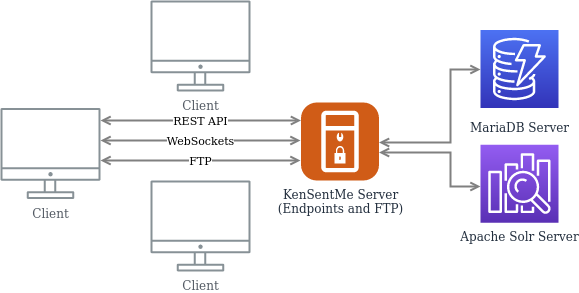
\includegraphics[width=0.75\linewidth]{imgs/arch.png}
 \caption{Software Architecture}
 \label{fig:arch}
\end{figure}

The KenSentMe server described in the previous figure provides different services, such as authentication, case resources, entity management, and others, as can be seen in Figure \ref{fig:services}.

\begin{figure}[ht]
 \centering
 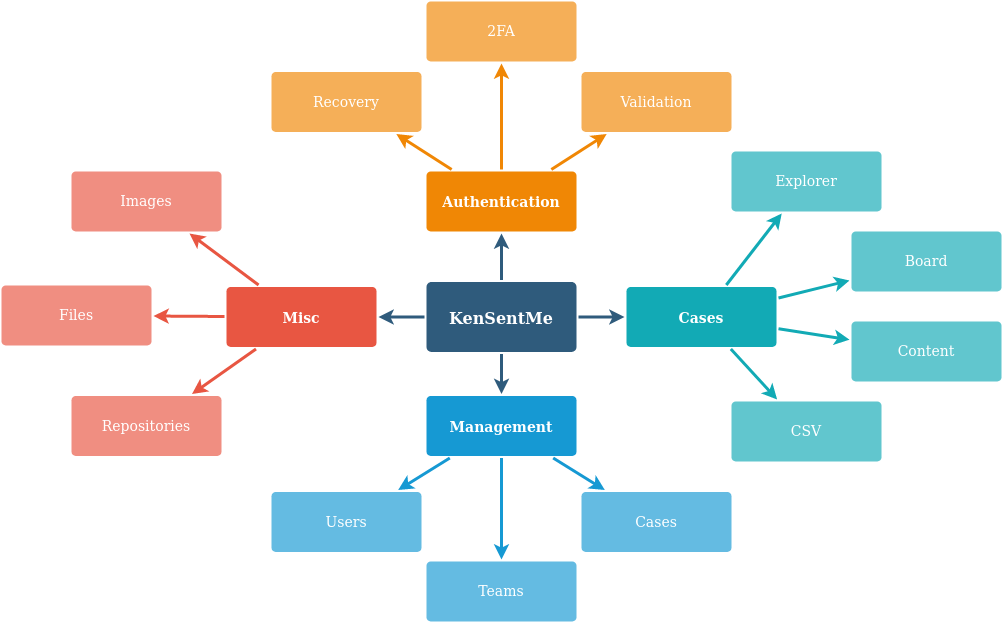
\includegraphics[width=1\linewidth]{imgs/services.png}
 \caption{Platform's Services}
 \label{fig:services}
\end{figure}

\section{Autopsy Source Code Analysis}

Autopsy is a digital forensics analysis software that is available as Open Source Software \cite{opensource} on \citetitle{github} \cite{github}.

With the goals set for this project, the source code was analyzed to understand which components need to be replicated and adapted in order to obtain the same logic flow.

The ``Core`` module is where the most important components are located, and after analysis it was concluded that the following directories present in Table \ref{tab:autopsyOverview} contain relevant information.

\begin{tabularx}{\textwidth}{@{}|c| *1{>{\centering\arraybackslash}X}@{}|}
    \hline
    \textbf{Name} & \textbf{Description} \\
    \hline\hline
    Actions & User interactions  \\
    \hline
    Casemodule & Case class and other resources needed for the functioning of an autopsy case like data sources and artifacts \\
    \hline
    Centralrepository & Data persisted and accessed by multiple cases (Correlation Engine) \\
    \hline
    Contentviewers & Panels used for data representation  \\
    \hline
    Coordinationservice & Configuration information distribution system \\
    \hline
    Core & Addition of command line options, system configurations and collaboration monitor  \\
    \hline
    Corecomponents & Main user interface components \\
    \hline
    Datamodel & All the entities needed to represent ingested data \\
    \hline
    Datasourceprocessors & Data processing utilities  \\
    \hline
    Directorytree & File explorer for ingested artifacts \\
    \hline
    Ingest & Utilities and events for data ingestion  \\
    \hline
    Keywordsearchservice & Utility to search artifacts by keyword  \\
    \hline
    Modules & All the pre-included modules (data ingestion procedures) \\
    \hline
    Progress & Progress indicators and similar classes \\
    \hline
    Python & Resources needed for the functioning of the Jython language \\
    \hline
    Rejview & Resources used to analyse Windows registry \\
    \hline
    Report & Report generation utilities and modules \\
    \hline
    Timeline & Recent addition to Autopsy, allows visualization of artifacts in temporal chart, only available for Windows OS \\
    \hline
    \caption{Autopsy Modules Overview}
    \label{tab:autopsyOverview}
\end{tabularx}

The ``KeywordSearch`` module is also of critical importance as it provides one of the most meaningful features which is filtering all the artifacts in a case with a keyword
search using the Apache Solr \cite{solr} search platform, which indexes the text contents of all the artifacts and allows extremely fast searching through a large amount of data.  

Another module that needs to be adapted is the ``RecentActivity`` module, which contains the tools needed to extract information from browsers, registry and other important resources, providing a great amount of
critical evidence from data sources.

Each autopsy case contains it's own SQLite \cite{sqlite} database, which contains the tables present in Table \ref{tab:tables}.

\begin{tabularx}{\textwidth}{|c|c|c|}
    \hline
    tsk\_db\_info & tsk\_db\_info\_extended & tsk\_objects \\
    \hline
    tsk\_image\_info & tsk\_image\_names & tsk\_vs\_info \\
    \hline
    tsk\_vs\_parts & tsk\_fs\_info & data\_source\_info \\
    \hline
    tsk\_files & file\_encoding\_types & tsk\_files\_path \\
    \hline
    tsk\_files\_derived & tsk\_files\_derived\_method & tag\_names \\
    \hline
    review\_statuses & blackboard\_artifacts & blackboard\_attributes \\
    \hline
    ingest\_modules & blackboard\_attribute\_types & ingest\_module\_types \\
    \hline
    reports & blackboard\_artifact\_types & ingest\_jobs \\
    \hline
    ingest\_job\_modules & ingest\_job\_status\_types & account\_types \\
    \hline
    accounts & account\_relationships & tsk\_event\_types \\
    \hline
    tsk\_examiners & blackboard\_artifact\_tags & content\_tags \\
    \hline
    tsk\_file\_layout & tsk\_event\_descriptions & tsk\_events \\
    \hline
    tsk\_pool\_info & & \\
    \hline
    \caption{Case Database Tables}
    \label{tab:tables}
\end{tabularx}

The tables containing the information accessed most frequently are the ones related to blackboard artifacts, along with tables related to files and tags.

Autopsy's source code allows access to most of the important entities present in this database, through pre-defined queries which return entities like data sources, abstract files, or artifacts. 
But in order to add features like pagination and tag deletion, custom queries must be created, so that the queries may return only a specific amount of entity ids, or so that delete commands may be executed. 

\section{Development Stages}

\subsection{Basic Autopsy Functionalities}

As a first step into replicating the functionalities of the original program, the most basic functionality from Autopsy was adapted, the ability to open an Autopsy case,  
as can be seen in Figure \ref{fig:open}.

\begin{figure}[ht]
 \centering
 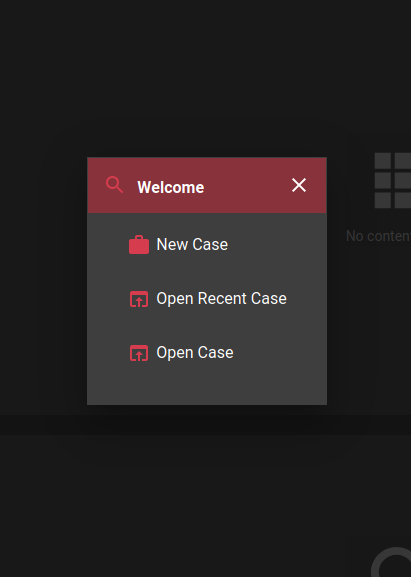
\includegraphics[width=0.35\linewidth]{imgs/welcome.png}
 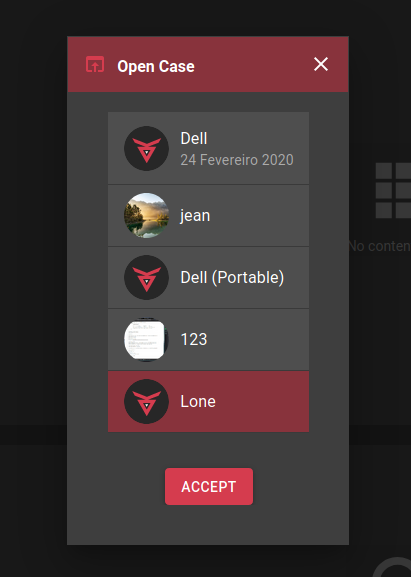
\includegraphics[width=0.35\linewidth]{imgs/open.png}
 \caption{Welcome and Open Case Modals}
 \label{fig:open}
\end{figure}

For this some elements of the original ''Casemodule'' package were adapted,
and after that all the other similar actions like closing, creating and deleting cases were also adapted.

Autopsy cases have a case file containing case metadata, which allows the program to connect to the right database when the case is open, this database is also present
in a file inside the file system, which uses the SQLite database engine. So for the cases to be usable in the server these files must also be present in the server,
which resulted in the creation of a directory within the server called ``repository``, containing all the different cases created within the application.

Later in the development there was the need to create an additional directory alongside the ``repository`` called ``central-repository``
which contains the database used by the Correlation Engine, which is a feature that finds files present in multiple cases, to ingest data that can be queried by any case.

The development of autopsy features was done with the original software as a reference, so that every new feature implemented into the platform could be compared and verified with the original software, and it was reassuring to see that cases created 
through one of the versions of the software were capable of being opened through the other version, meaning that the source code provided by autopsy, with some tinkering, can definitely be used in a client-server model.

\subsection{Authentication Process}

The authentication process is handled through a REST API, when the authentication is completed the user receives a JSON Web Token (JWT).

JWT is an open standard that defines a compact and self-contained way for securely transmitting information between parties. This information can be verified and trusted because it is digitally signed.
JWT contain three parts, as can be seen in Table \ref{tab:jwtComposition}.

\begin{table}[ht]
  \begin{tabularx}{\textwidth}{@{}|c| *1{>{\centering\arraybackslash}X}@{}|}
    \hline
    \textbf{Name} & \textbf{Contents} \\
    \hline\hline
    Header & Information about the signing algorithm used  \\
    \hline
    Payload & Information about the user, such as username, e-mail and roles \\
    \hline
    Signature & A signature used to verify the contents weren't changed \\
    \hline
  \end{tabularx}
  \caption{JWT Composition}
  \label{tab:jwtComposition}
\end{table}

The authentication can be performed with either username or e-mail and a password, and extra authentication factors can be added such as One Time Passwords (OTP) and Universal Second Factor (U2F).

If no extra factors were added to an account, the authentication attempt with the user's credentials will return the JWT when successful and the user can freely access protected content.

When extra factors are present in an account, the response from the same request will contain an array with the extra factors added, and a UUID, which is a pseudo random string, which must be sent in the next request to validate the user's identity.

This UUID is saved in the database in the form of salted hash using the Blowfish \cite{blowfish} algorithm, and is invalidated after a successful login attempt. The user then has the choice between any of the extra factors and must complete the required steps to validate that factor, as can be seen in Figure \ref{fig:login}.

\begin{figure}[ht]
 \centering
 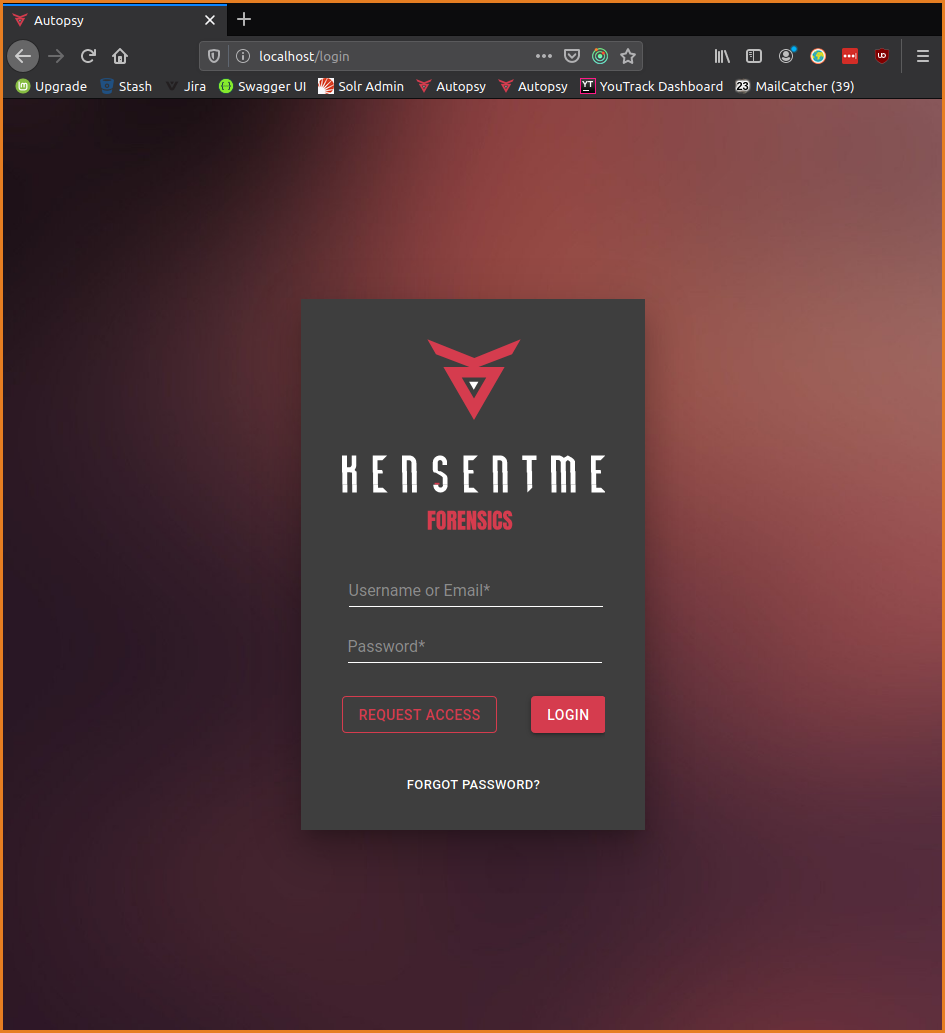
\includegraphics[width=0.35\linewidth]{imgs/login.png}
 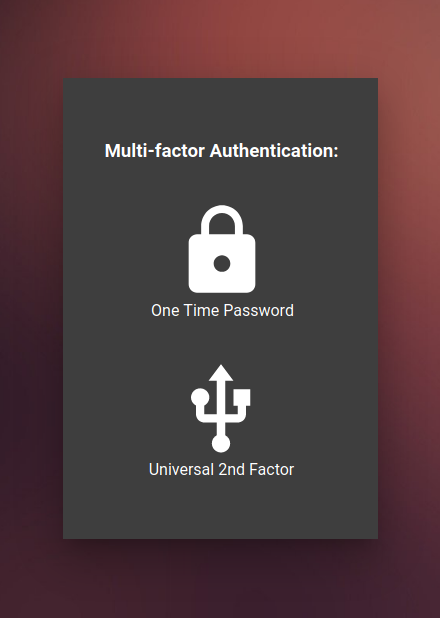
\includegraphics[width=0.35\linewidth]{imgs/mfa.png}
 \caption{Login Screen and Extra Factors}
 \label{fig:login}
\end{figure}

\subsubsection*{One Time Password}

The process of setting up OTP for an account begins with generating a secret string, which is used by both the server and the authenticator app to generate OTP, when the secret is generated, it is saved as a temporary secret after being encrypted by the RSA algorithm.

The temporary secret must be added to the user's device, either by inserting the string itself or by scanning a QR code \cite{qr}, and must be validated by the user by submitting the current OTP, after validation the temporary secret is considered permanent.

All OTP validations have a 30 second threshold, which means the current OTP is valid for an extra 30 seconds after being replaced by the next OTP, allowing the user to have a better experience with these passwords.

The processes of authenticating and removing this authentication factor both depend on validating the current OTP, which is provided by the user's app.

In the event of loss of the device that the user uses to generate OTP, all the authentication factors can be reset using the ''Reset Password'' functionality, which relies on e-mail validation to prove the user's identity.

\subsubsection*{Universal Second Factor}

Both the set up and validation of U2F are very similar, as these procedures require the server to generate a challenge.
This challenge is transmited to the client, and then transmited to the U2F device, which then generates the response which is used to validate the challenge.

In the case of setting up the device, if the response is validated successfully, the information present in Table \ref{tab:u2f} is stored in the server and the procedure is completed.

%TODO SHOULD NOT BE NEEDED PAGE BREAK
\pagebreak

\begin{table}[ht]
  \begin{tabularx}{\textwidth}{@{}|c| *1{>{\centering\arraybackslash}X}@{}|}
    \hline
    \textbf{Name} & \textbf{Description} \\
    \hline\hline
    Key Handle & Identification of the registration, allows the same key to be used for multiple accounts in the same domain  \\
    \hline
    Public Key & Resulting from the generation of a key pair specific to the domain, used to verify the information provided by the device \\
    \hline
    Attestation Certificate & A certificate that can be used to verify the authenticity of the device \\
    \hline
    Counter & The device's authentication counter, used to prevent the use of cloned devices \\
    \hline
    Compromised & Flag indicating if the credential is considered to be compromised \\
    \hline
  \end{tabularx}
  \caption{U2F Registration Composition}
  \label{tab:u2f}
\end{table}

When authenticating the challenge depends on the public key previously stored, which means only the device used to set up can generate the right response to the challenge.

The U2F procedure is represented in Figure \ref{fig:yubi}.

\begin{figure}[ht]
 \centering
 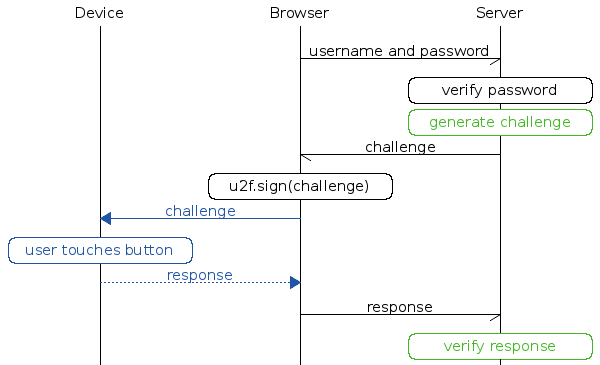
\includegraphics[width=1\linewidth]{imgs/yubi.png}
 \caption{U2F Procedure \cite{yubi}}
 \label{fig:yubi}
\end{figure}

\subsection{Management Entities}

Further in the development, the different persisted entities were created, which are Users, Teams, and Cases. All the endpoints for actions involving these 
entities were created, resulting in the ability for the client program to interact with these entities and modify their relationships and other variables.

For these functionalities there are two roles associated, (1) the Manager role allows manipulation of the existing entities while (2) the Investigator role only has access to his
own information and the teams and cases he was assigned to. For these interactions, it was decided to create a drag and drop interface, which allows users to be dragged into
teams and teams dragged into cases. All these entities are listed side by side and each have their own options and filtering input, as can be observed in Figure \ref{fig:users}.

\begin{figure}[ht]
 \centering
 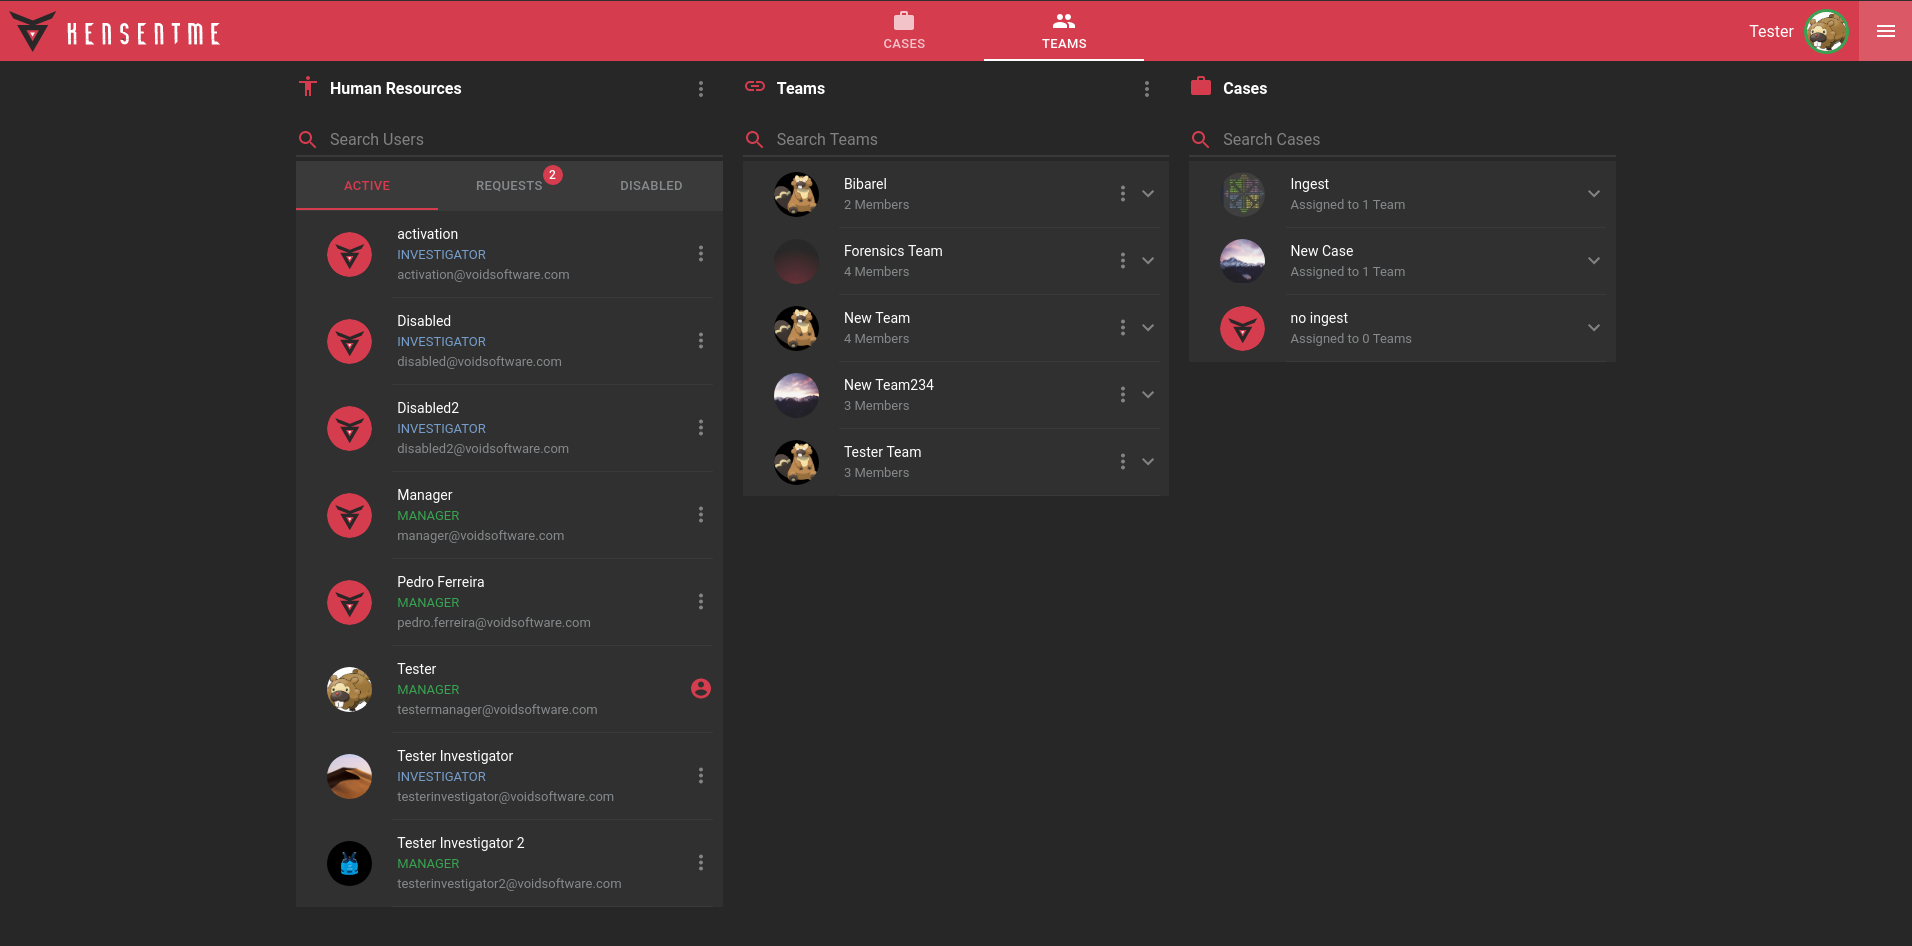
\includegraphics[width=1\linewidth]{imgs/users.png}
 \caption{Entity Management Interface}
 \label{fig:users}
\end{figure}

Users can change their own profile picture, while Managers can also change any team or case's display picture.

Managers can add new users to the platform, can approve membership requests, can enable/disable user accounts and can create new teams.

When a user is added by a Manager or his membership request is approved, he must define a password when activating his account through a received e-mail message.

It was at this step in development that was made clear by the testers, that validations must be preformed on both server and client side, and that error handling must be streamlined
in order to provide a seamless experience to the user, while also allowing future additions to the platform to be implemented in a similar way without much tinkering.

Because even though the platform still wasn't fully developed, it already suffered from possible exploits that could break the experience for it's users, like the upload of a 5GB file
as an image file, which would stop the page from loading, or possible directory traversal attacks, resulting from the creation of case directories.

The lessons learned from the testers on this stage of development carried on through the entire development process and ensured that every new feature added was accounting for possible weaknesses which may result from the new 
implementations, resulting in a more secure development process.

The platform's resulting data model can be observed in Figure \ref{fig:database}.

\begin{figure}[ht]
 \centering
 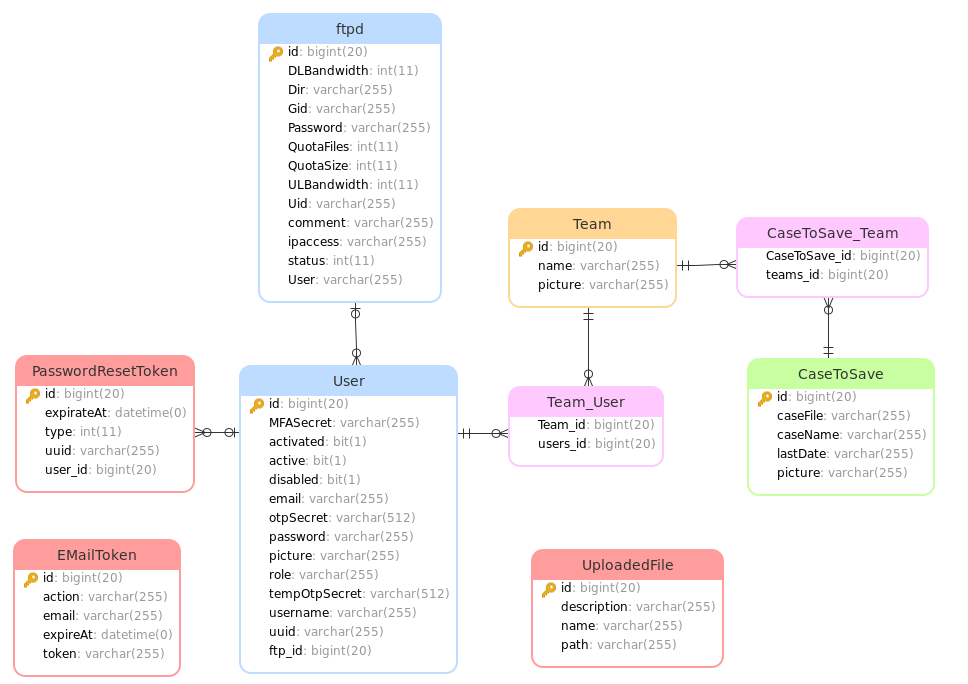
\includegraphics[width=1\linewidth]{imgs/database.png}
 \caption{Database Structure}
 \label{fig:database}
\end{figure}

\subsection{Ingested Results Presentation}

Ingested results are the items present inside the provided data sources. Autopsy can run multiple modules on each data source to extract results, and the extracted results can either be a file instance or an artifact instance.
The difference between a file and an artifact is that an artifact represents only a smaller piece of a file's information, which means a file can contain multiple artifacts, for example a registry file can contain multiple OS user account artifacts.

Even though the data ingestion features weren't implemented yet on the platform, the data that was ingested into a case using the original program could also be used on this platform, which allowed this feature to be developed earlier.

The ingested results are presented in three different containers, one taking the shape of a file explorer, allowing exploration of the structure of all the results, 
one taking the shape of a table or thumbnail viewer, that can be referenced as a board, presenting all the contents of the results selected from the explorer, and one taking the shape of a content viewer, allowing visualization
of the data contained inside the result selected from the table as can be seen in Figure \ref{fig:data}.

\begin{figure}[ht]
 \centering
 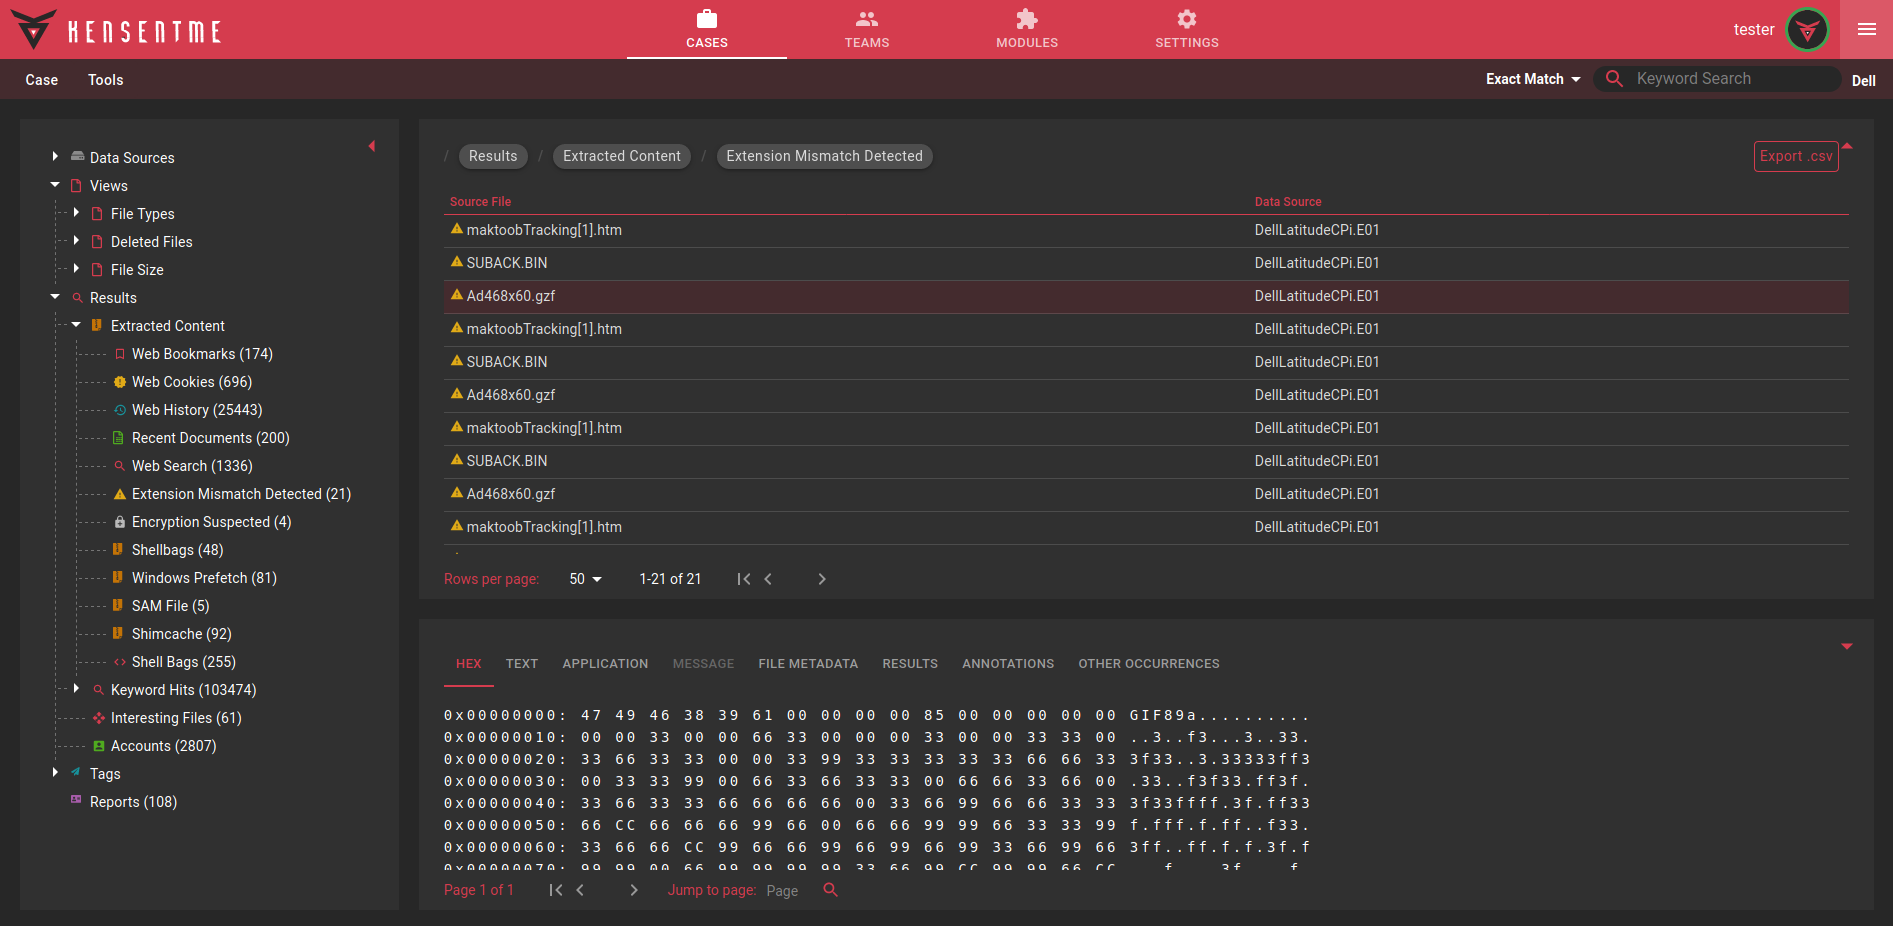
\includegraphics[width=1\linewidth]{imgs/data.png}
 \caption{Ingested Results Presentation (A) Explorer; (B) Board; (C) Content Viewer}
 \label{fig:data}
\end{figure}

The content viewer can display different kinds of information depending on the type of item selected, these can be some of the following:
\begin{itemize}
 \item Text browser
 \item Media viewer
 \item Database browser
 \item Registry browser
 \item Key-value browser
 \item Table data viewer
\end{itemize}

The layout for the ingested results presentation, and for all the case related actions, was based on the original Autopsy layout, so that each container can be re-sized as
needed, allowing the user to focus on the information that is most important to him.

This development stage was one of the most intensive, as it required understanding Autopsy's data structure very well. The source code used here was rewritten almost completely, 
because of the way the user interface and the data structure in the original program are interconnected, resulting in the need to adapt and write custom queries to obtain the desired results (which include pagination), creating 
65 endpoints so that all the needed information could be supplied, as well as creating and adjusting all the UI elements to achieve an user experience similar to what Autopsy's users are used to.

\subsection{Tag Management}

Tagging content is a very important step in forensics investigations, as it allows the investigators to keep an organized list of important information.

Tagging was added to the platform in the form of a context menu, that is shown by selecting information from the table/thumbnail viewer, as can be seen in Figure \ref{fig:tags}.

\begin{figure}[ht]
 \centering
 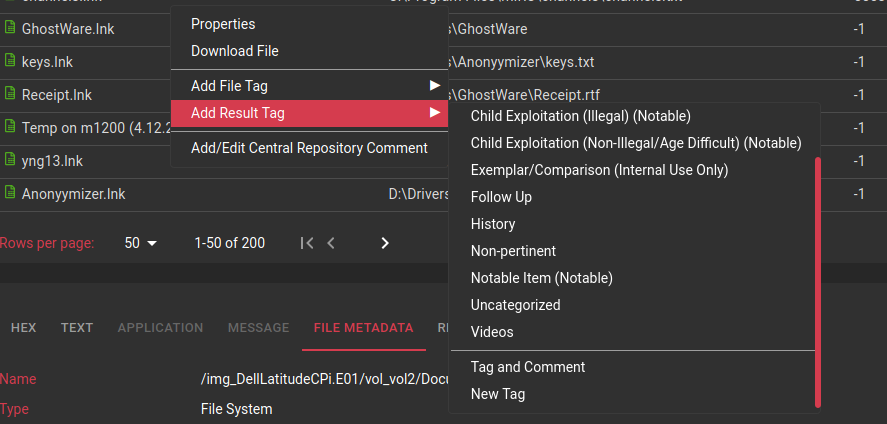
\includegraphics[width=1\linewidth]{imgs/tags.png}
 \caption{Tags Context Menu}
 \label{fig:tags}
\end{figure}

Tags take the form of file or result tags, and the difference is that a result tag is specific to an artifact, while a file tag is related to the file itself.

Autopsy contains 10 different tag types by default, and more can be added, which can result in a high amount of tag types in use, which deteriorates the user experience.

Tag names are also shared between cases, so it seemed important to have more control over the management of these tags, and the ability to delete tag types was added, even though it didn't exist in the original software.

Since each case contains it's own database, it's impossible to synchronize every case at once when a tag is deleted, so it was necessary to create a procedure to synchronize case tags when a case is opened.

\subsection{Data Sources}

Using the same credentials used to log-in to the platform, the user can also upload data source files into his folder located inside the server, using an FTP client like FileZilla \cite{filezilla}.
Then the user can browse these directories using the web interface and select a data source to add to the case, as can be seen in Figure \ref{fig:datasource}.

\begin{figure}[ht]
 \centering
 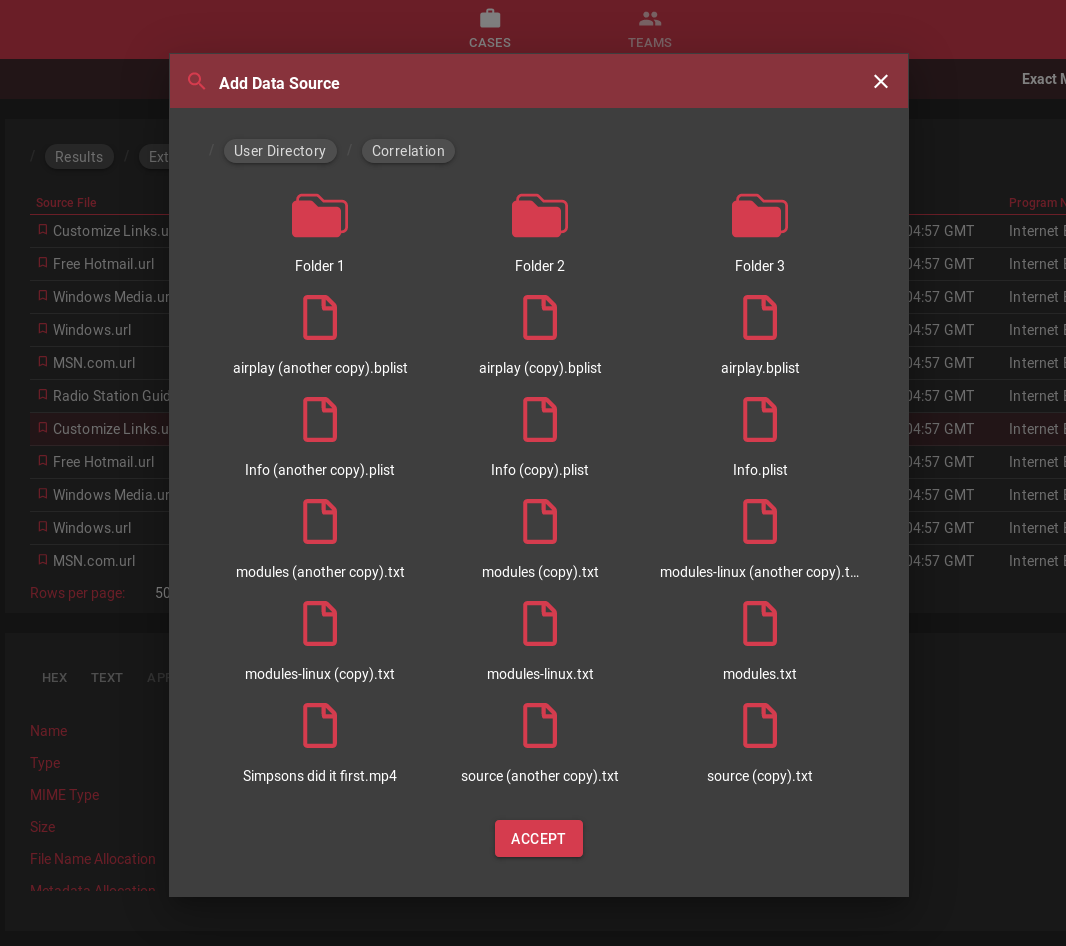
\includegraphics[width=0.75\linewidth]{imgs/data-sources.png}
 \caption{Data Source Selection}
 \label{fig:datasource}
\end{figure}

The procedure for adding a data source to a case was adapted from Autopsy's source code, and depends on the type of data source added, which can be one of the following:
\begin{itemize}
 \item Disk image
 \item Virtual machine
 \item Logical file collection
 \item Autopsy logical imager results
\end{itemize}

Local disk data sources were also an option provided by Autopsy but since the local disks the software has access to belong to a server, this feature is undesired.

When a data source is added to a case, it is processed and instances of abstract files and other entities are created, which allow the user to navigate the data source's contents as soon as it is processed.

Just navigating the data source contents isn't very useful, as the contents are in a raw state, showing mostly the file structure of the source, and not even categorizing files by mime types, so running data
ingestion modules is a critical step into allowing a deeper analysis of a data source, which is covered in the next section.

\subsection{Data Ingestion Modules}

Data ingestion modules can be either file ingest modules, which analyse each file contained in a data source, one by one,
or data source ingest modules, which run on specific components of a data source.

To run a collection of modules, the user selects which modules to run, and may also configure some parameters related to the modules, when the request is received by the server, the modules are started in a background thread.

When the modules are running the server communicates to each client through WebSockets, offering feedback on the progress of the modules, as can be seen in Figure \ref{fig:modules}.

\begin{figure}[ht]
 \centering
 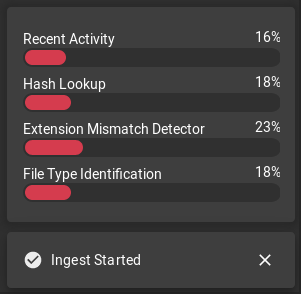
\includegraphics[width=0.55\linewidth]{imgs/modules.png}
 \caption{Ingest Modules Communication}
 \label{fig:modules}
\end{figure}

Originally it was intended to have the clients update their explorer as new information is ingested, but it would slow down the ingest progress considerably, so what was decided was that every client would refresh 
it's explorer every 30 seconds while ingests are running.

There were other measures taken into consideration to improve the performance of the ingest procedure, while also maintaining the user informed of it's progress, the server communicates a maximum of one file name per
second, and it also only communicates a module's progress when it advances at least one percentage point.

\subsection{Report Modules}

Report modules consist in generating a file or collection of files, to further process, filter, or present the results found in a case. They can take many shapes such as a text file, spreadsheets, HTML pages or even a portable case that can be imported into Autopsy.

Report modules have the ability to process existing data and generate results based on that, such as validating e-mail addresses or credit card numbers, 
which are found based on regular expressions by the keyword search module and may contain false positives.

The adaptation of the source code for report modules went pretty smoothly, with the exception that some modules require the user to provide a file when running the module, which resulted in the creation of a file repository within the server, for files to be used in this manner.

\subsection{Add-on Modules}

Autopsy supports third party modules in the form or NetBeans \cite{netbeans} module files (NBM), and in the form of python scripts, using the Jython language, which allows python code to run alongside classes defined in Java.

Since the developed platform doesn't support a java user interface, the procedure to install Netbeans modules could not be implemented, as this feature is specific to Netbeans applications. 
But most modules are made in the Jython language, and the addition of this modules was implemented as intended.

A user with a manager role can add new modules to the platform by either selecting from defined repositories or by uploading a zip archive containing the modules, as can be seen in Figure \ref{fig:addmodule}.

\begin{figure}[ht]
 \centering
 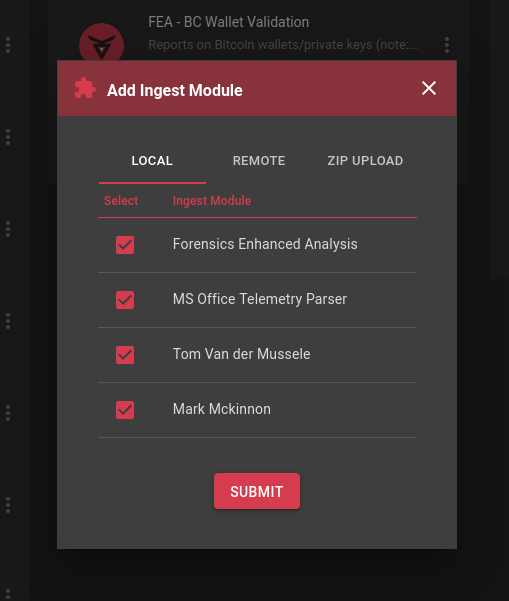
\includegraphics[width=0.55\linewidth]{imgs/addmodule.png}
 \caption{Add-on Modules Addition}
 \label{fig:addmodule}
\end{figure}

These repositories previously mentioned can be defined in the platform itself, or accessed from a remote source, which is a standalone platform developed just for this purpose and could allow the company to provide repository sources to any deployed version of the platform.

The platform also allows management of the added modules, so that managers can enable, disabled and remove certain modules, as can be seen in Figure \ref{fig:modulesettings}.

\begin{figure}[ht]
 \centering
 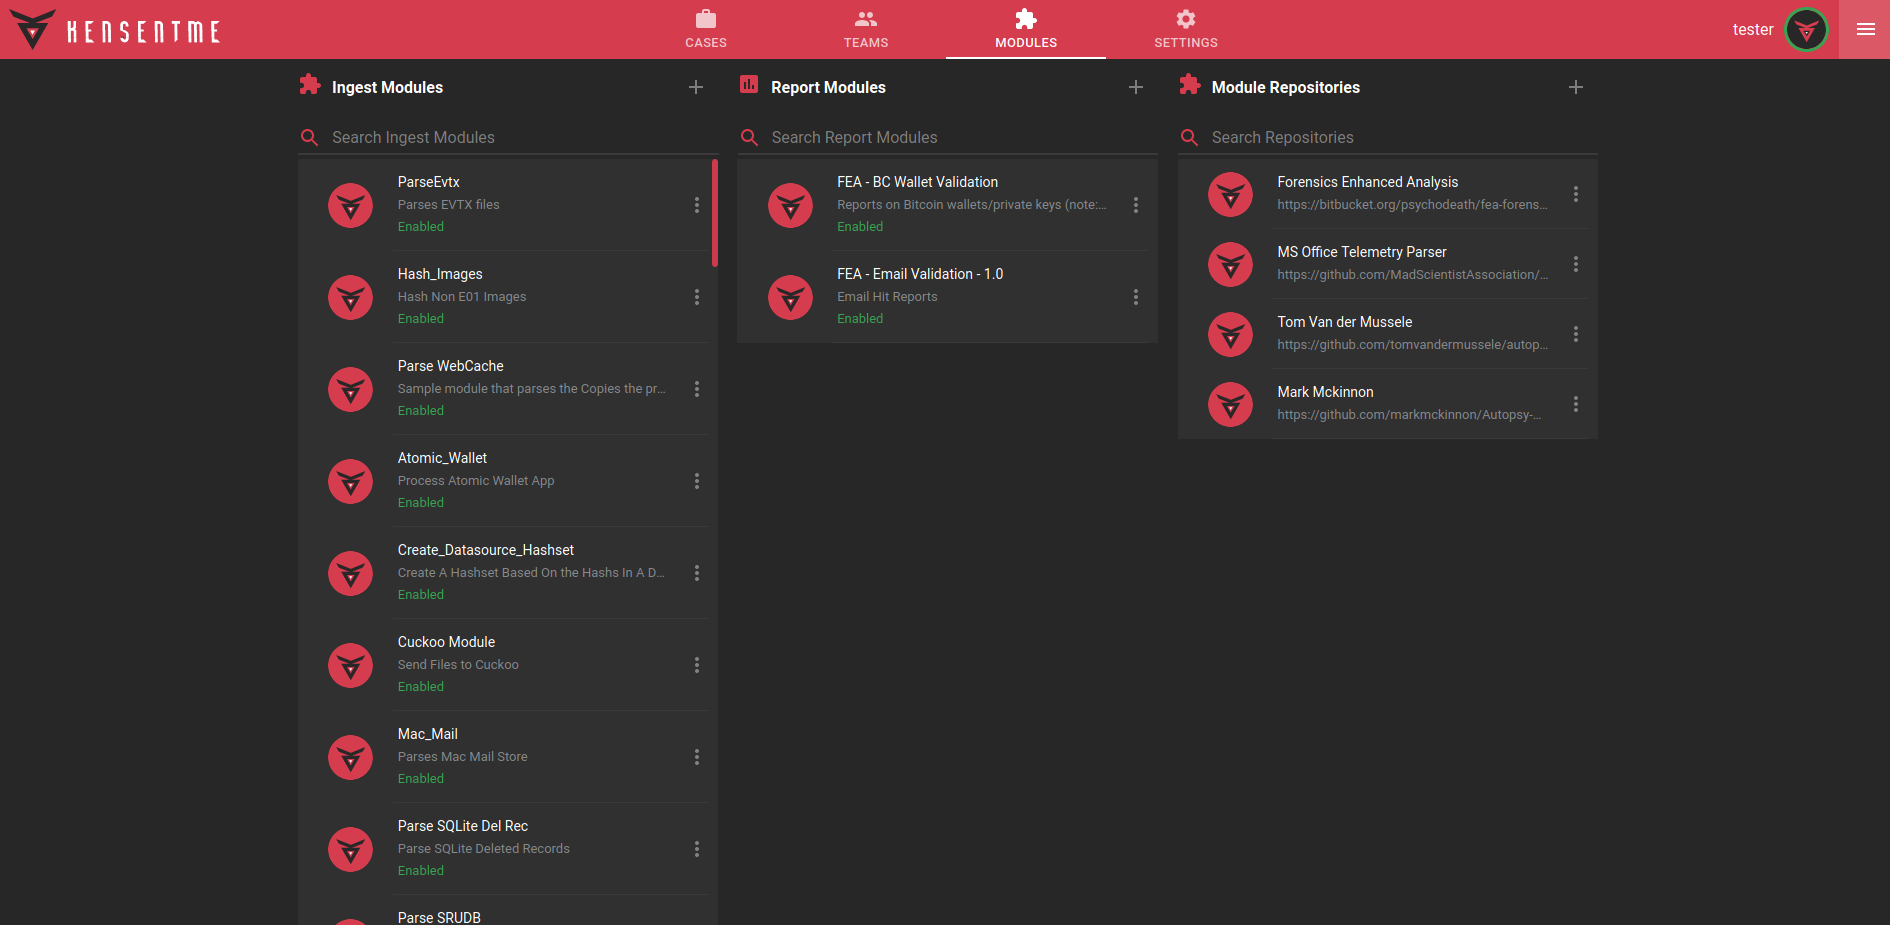
\includegraphics[width=1\linewidth]{imgs/modulesettings.png}
 \caption{Add-on Modules Management}
 \label{fig:modulesettings}
\end{figure}

Third party modules require that a great deal of the original Autopsy source code is accessible in the original namespace, which resulted in the separation of the
developed and adapted code into two different namespaces, the original software's namespace which is org.sleuthkit.autopsy, and the company's namespace which is pt.voidsoftware.kensentme. 

This requirement of the original code can also mean that some modules which weren't tested may fail to run due to missing code, but a procedure to handle failure to run modules is implemented, 
and it informs the user about which modules are failing to run, allowing the user to disable the unsupported modules.

\subsection{Project Deployment and Documentation}

A ''Read Me'' document was created, detailing each step required to setup the platform, which involves installing all the dependencies required, as well as compiling the developed code.

The setup was tested in multiple versions of Linux and with different versions of needed dependencies, resulting in a controlled step-by-step guide that can be followed in about 30 minutes that leads to a successful deployment of the complete platform.

The documentation of every endpoint of the platform can be consulted in \autoref{ch:appendixA}.

\section{Critical Analysis and Proposed Improvements}

The development of the platform halted due to it being considered in a finished state, which means that all the objectives for the project were completed successfully.

Given that Autopsy is still in active development, it would be very important to keep following it's development, and complementing this platform with new features and bug fixes which might come up in the future.

Besides accompanying Autopsy's improvements, it could also be interesting to further develop the platform to better serve the needs of it's users, which would require installations of the platform, and a feedback channel to better understand the user's needs.

%\cleardoublepage\addtocontents{toc}{\protect\vspace{\beforebibskip}} % Place slightly below the rest of the document content in the table


%************************************************
\chapter{Other Projects Developed}
\label{ch:projects}
%************************************************

\section{IGiveU}

\subsection{Critical Analysis and Proposed Improvements}

\section{Another Project?}

\subsection{Critical Analysis and Proposed Improvements} 
\cleardoublepage\addtocontents{toc}{\protect\vspace{\beforebibskip}} % Place slightly below the rest of the document content in the table


%************************************************
\chapter{Conclusões}
\label{ch:conclusoes}
%************************************************


O uso do \LaTeXe permite-nos focar no essencial: o conteúdo, a formatação é tratada de forma automática.

Para mais informações sobre o \LaTeXe aconselha-se a consulta do
livro \emph{The Not So Short Introduction to \LaTeXe}~\cite{oetiker2000nss}.

Para a gestão de referências bibliográficas aconselha-se o JabRef. %\cite{jabref}.
 

\cleardoublepage%********************************************************************
% Bibliography
%*******************************************************
% work-around to have small caps also here in the headline
\manualmark
\markboth{\spacedlowsmallcaps{\bibname}}{\spacedlowsmallcaps{\bibname}} % work-around to have small caps also
\phantomsection 
\refstepcounter{dummy}
\addtocontents{toc}{\protect\vspace{\beforebibskip}} % to have the bib a bit from the rest in the toc
\addcontentsline{toc}{chapter}{\tocEntry{\bibname}}

\printbibliography
\label{app:bibliography} 


%********************************************************************
% Backmatter
%*******************************************************
\appendix

\cleardoublepage
\phantomsection 
\part*{Appendices}
% 
\cleardoublepage\addtocontents{toc}{\protect\vspace{\beforebibskip}} % Place slightly below the rest of the document content in the table

% If problems with the headers: get headings in appendix etc. right
\markboth{\spacedlowsmallcaps{Anexos}}{\spacedlowsmallcaps{Anexos}}

% Appendix A
%\chapter{Appendix A}
%\label{ch:appendixA}
%The endpoints of the KenSentMe platform are presented in the following pages, using the Swagger tool.

%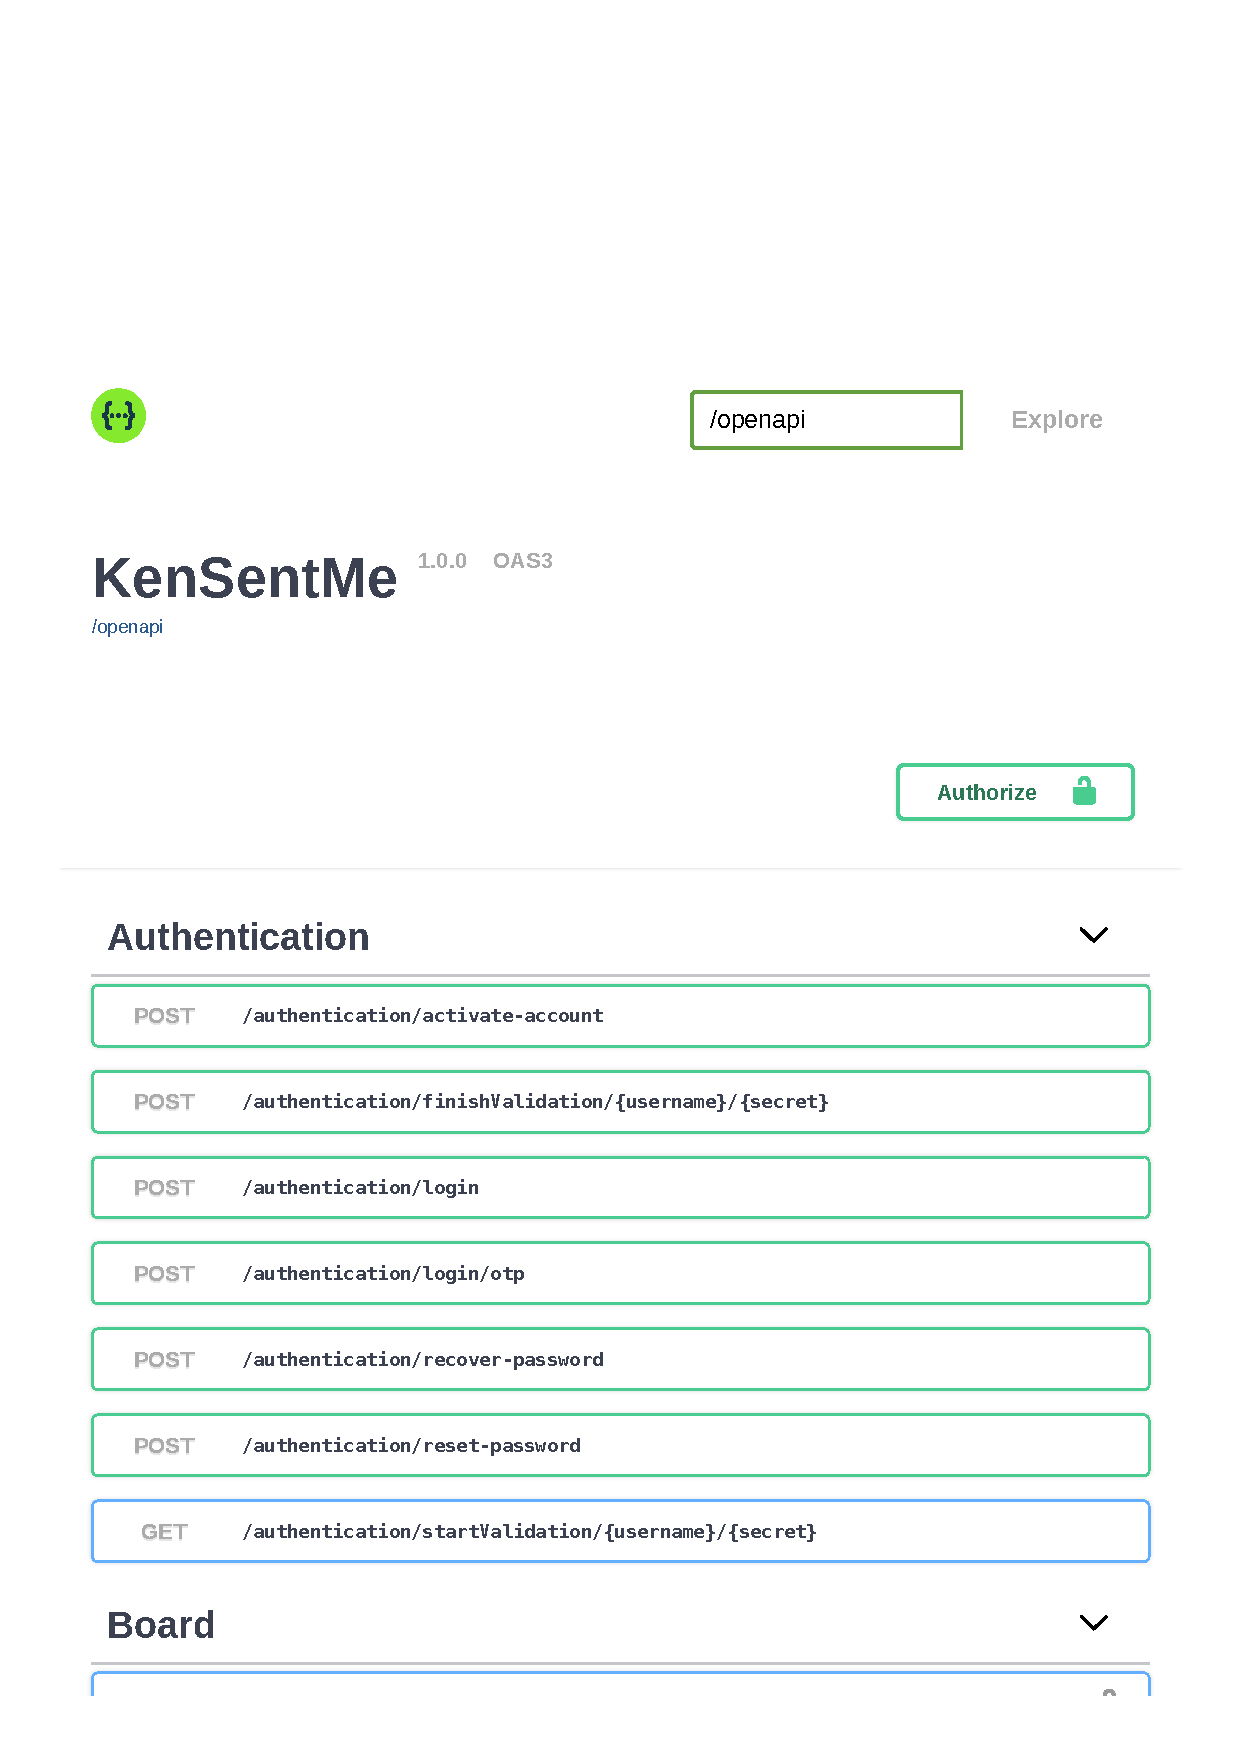
\includepdf[pages=-,width=1.25\textwidth]{pdfs/swagger.pdf}

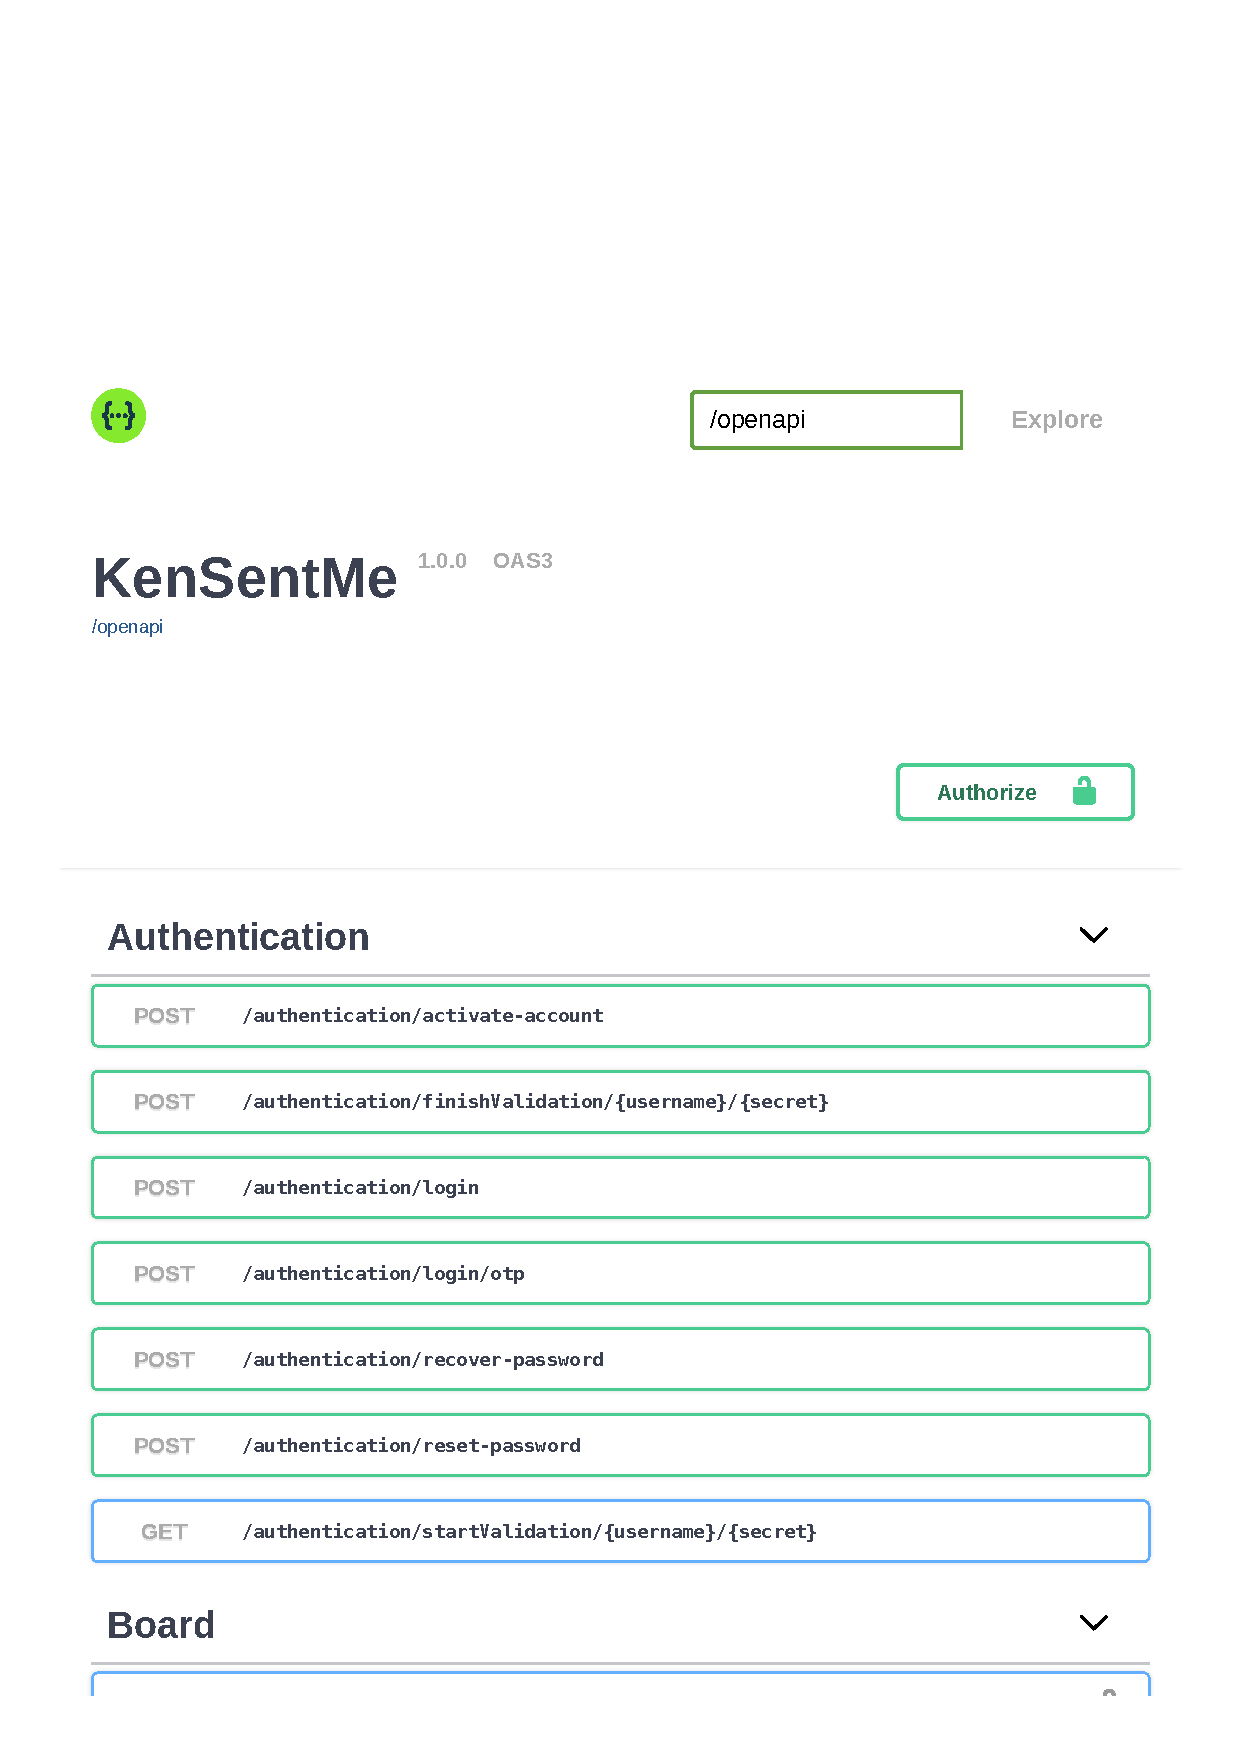
\includepdf[pages=1,pagecommand={\chapter{Appendix A} \label{ch:appendixA} The endpoints of the KenSentMe platform are presented in the following pages, using the Swagger tool.}, width=1.25\textwidth]{pdfs/swagger.pdf}
\includepdf[pages=2-,width=1.25\textwidth]{pdfs/swagger.pdf}

% 
\cleardoublepage\addtocontents{toc}{\protect\vspace{\beforebibskip}} % Place slightly below the rest of the document content in the table

% Appendix X
\chapter{Appendix B}
%----------------------------------------------------------------------------------------

% Content begins here


\lipsum[15]



\cleardoublepage%*******************************************************
% Declaration
%*******************************************************


\refstepcounter{dummy}
\addtocontents{toc}{\protect\vspace{\beforebibskip}} % to have the bib a bit from the rest in the toc
\addcontentsline{toc}{chapter}{\tocEntry{Declaração}}
\chapter*{Declaração}
\thispagestyle{empty}


Declaro, sob compromisso de honra, que o trabalho apresentado nesta dissertação, com o título \textit{``\myTitle''}, é original e foi realizado por \myNameOne (\myNumber) sob orientação de \myProfOne.

\vspace{15 mm}

\noindent\textit{\myLocation, \myTime}
\bigskip

\begin{flushright}
    \begin{tabular}{m{8cm}}
        \\ \hline
        \centering\myNameOne \\
    \end{tabular}
\end{flushright}

% \vspace{5 mm}
% 
% \begin{flushright}
%     \begin{tabular}{m{8cm}}
%         \\ \hline
%         \centering\myNameTwo \\
%     \end{tabular}
% \end{flushright}




% 
% \begin{flushright}
%     \begin{tabular}{|m{10cm}}
%         \\ 
%         \centering  %\myName \\
%     \end{tabular}
% \end{flushright}
% 
% \vspace{5 mm}
% \begin{flushright}
%     \begin{tabular}{|m{10cm}}
%         \\ 
%         \centering  %\myName \\
%     \end{tabular}
% \end{flushright}
% 
% 

%********************************************************************
% Game Over: Restore, Restart, or Quit?
%*******************************************************
\end{document}
%********************************************************************
